% DIV Grösser -> Mehr Text pro Seite
% Bindekorrektur BCOR
% A5
%\usepackage[a5paper,BCOR12mm]{typearea}

\usepackage{kpfonts}
\usepackage{ucs}

% Load symbols like «»
\usepackage[T1]{fontenc} % Load amsmath before this! http://en.wikibooks.org/wiki/LaTeX/Internationalization#Cyrillic_script
% Then load additional utf8 symbols + encoding
\usepackage[utf8x]{inputenc}
\usepackage[russian,ngerman]{babel}

\usepackage{DejaVuSerif}
\newcommand{\ru}[1]{\usefont{T1}{DejaVuSerif-TLF}{m}{n} {\selectlanguage{russian} #1 \selectlanguage{ngerman} \fontfamily{cmr}\selectfont}}
\renewcommand{\rmdefault}{cmr}

\usepackage{xcolor}
\usepackage{fontenc}
\usepackage{graphicx}

\usepackage[dvips,pdftex,pdfusetitle]{hyperref}

% Math environments
\usepackage{amsmath}
\usepackage{amsfonts}

\usepackage{calc}

% For top/mid/bottomrule
\usepackage{booktabs}

\usepackage{xtab}
\usepackage{longtable}
\usepackage{tabu}
\usepackage{colortbl}

\usepackage{rotating}
\usepackage{varwidth}

\usepackage{wrapfig}
\usepackage{multicol}

% Colored headers
\usepackage{sectsty}

\definecolor{seccol}{cmyk}{.8,0,0,.6}
\allsectionsfont{\color{seccol}}

%\usepackage{cclicenses}

\newcommand{\imgsrc}[1]{ { \small \textit {#1} }}

\definecolor{linkcol}{cmyk}{0,.58,.93,.29}
\newcommand{\plink}[2]{{\color{linkcol}\textbf{›}\hyperref[#1]{#2}, Seite \pageref{#1}}}
\newcommand{\tlink}[2]{{\color{linkcol}\textbf{›}\hyperref[#1]{#2}:\pageref{#1}}}

\definecolor{samplecol}{cmyk}{.28,0,.91,.28}
\newcommand{\cw}[1]{{\color{samplecol}\texttt{#1}}}

\newcommand{\call}[1]{\texttt{#1}}


% Bash
% Table LibO -> LaTeX
% cat file.txt |sed -e 's/\t/ \& /g' |perl -p -e 's/$/ \\\\/'

\title{Amateurfunkbehelf}
\author{Simon A. Eugster}
\date{}

\pdfinfo{%
  /Title    (Amateurfunkbehelf)
  /Author   (Simon A. Eugster)
  /Creator  ()
  /Producer ()
  /Subject  ()
  /Keywords ()
}

\definecolor{rowsep}{gray}{.7}

\newcommand{\link}[1]{::#1}

\newcommand{\lit}[1]{
\noindent
\begin{minipage}{\textwidth}
 \parbox[t]{2em}{ \raisebox{-0.5mm}{
\includegraphics[height=1em]{./png/Amfu-Icon-Buch.png}} }
 \parbox[t]{\dimexpr \textwidth-2.5em}{#1}
 \vspace{.5em}
\end{minipage}
}

% \toprule width
\setlength{\heavyrulewidth}{.1em}

\begin{document}

\begin{titlepage}
 \begin{center}
 \vspace*{2cm}
 
 
 
\includegraphics{./png/Amfu-Logo_Anja.png}
 
 \vspace*{4cm}
 
 % Full page width; http://tex.stackexchange.com/questions/265/fonts-larger-than-huge
% \resizebox{\linewidth}{!}{Amateurfunkbehelf}

 {\textsc{\usefont{T1}{DejaVuSans-TLF}{b}{n}  \fontsize{28pt}{28pt}\selectfont Behelf}} \hfill \hspace{\stretch{1}} \\
 {\vspace{8pt} \textsc{\usefont{T1}{DejaVuSans-TLF}{b}{n}  \fontsize{40pt}{40pt}\selectfont Amateurfunk}} \hfill \hspace{\stretch{1}}
 %\HUGE{Behelf}\\ Amateurfunk
 
\end{center}
\end{titlepage}

{
\usefont{T1}{DejaVuSans-TLF}{m}{n}

\cleardoublepage
\vspace*{3cm}
\noindent
Copyright (c) \hspace{1em} 2008--2013 \hspace{1em} hb4ff Operators and Authors.

\vspace{1em}
\noindent
Permission is granted to copy, distribute and/or modify this document\\
under the terms of the \textbf{GNU Free Documentation License,} Version 1.3\\
or any later version published by the Free Software Foundation;\\
with no Invariant Sections, no Front-Cover Texts, and no Back-Cover Texts.\\
A copy of the license is included in the section entitled «GNU\\
Free Documentation License».

\vspace{2em}
\noindent
Dieser Behelf sowie die Karten, Grafiken und Vorlagen \\
können unter \textit{\href{http://ham.granjow.net}{http://ham.granjow.net}} heruntergeladen werden.

\vspace{2em}
\noindent
Die Autoren übernehmen keine Haftung \\
für in Zusammenhang mit diesem Dokument entstandene Schäden.\\
Der Leser handelt in eigener Verantwortung.\\

\cleardoublepage
\vspace*{3cm}
\begin{centering}
Dieser Behelf wurde von Amateurfunkern der Station HB4FF\\
ins Leben gerufen.

\vspace{1em}
Diese Ausgabe ist vom \today.

\vspace{2em}
\textbf{Autoren}\\ \vspace{4pt}
Jannick Griner\\
Jürg Rüfli, hb9bfc\\
Markus Walter, hb9hvg\\
Simon A. Eugster, hb9eia

\newcommand{\dank}[2]{\vspace{4pt}#1\\{\footnotesize #2} \\}
\vspace{2em}
\textbf{Dank}\\
\dank{Anja Ballschmieter}{für das Logo auf der Titelseite}
\dank{Stephan Bolli, hb9tnp}{für die HB9-Formelsammlung}
\dank{Paul-Adrien Braissant, hb9cuf}{für die Hinweise und Ergänzungen zu Modulation und Verfahren}
\dank{Josef Buchs, hb9mty}{für die ergänzenden Beschreibungen der Modulationsverfahren}
\dank{Karl Haab, hb9aiy}{für die technischen Ergänzungen}
\dank{Peter Kumli, Bakom}{für die Bereitstellung der Vorschriften}
\dank{Oona Svan}{für die Grafik mit dem Maidenhead-Locator}
\dank{Renato Schlittler, hb9bxq}{für die Relaislisten}
\dank{Gregor Wuthier, hb9dmh}{für die Anregungen zum Inhalt}
\end{centering}

}

\tableofcontents

\chapter{Vorwort}
Das Ziel dieses Behelfs ist es, wichtige Informationen in kompakter Form bereitzustellen, speziell für mobilen oder portablen Einsatz\footnote{Am praktischsten ist er im Format A5.} (Ermöglicht wird dies auch durch die bereitgestellten Anhänge, wofür wir uns bedanken). Er ist aus den Grund entstanden, dass schlicht und einfach die Notwendigkeit daran bestand, aber noch nichts dergleichen existierte.

\section{Lizenz}
Frei zugängliches Wissen ist die Zukunft, wie auch die Wikipedia beweist. Aus diesem Grund steht dieser Behelf (inklusive Grafiken) und unter der GFDL, der GNU Free Documentation License. Das heisst unter anderem, dass er auch abgeändert und weiterverwendet werden darf (etwa für andere deutschsprachige Länder), unter der Bedingung, dass er weiterhin unter dieser Lizenz stehen muss. Genaueres unter \plink{sec:gfdl}{GNU Free Documentation License}.

\section{Prüfung}
\lit{Amateurfunk-Lehrgang von Eckart Moltrecht. Drei Bücher, auch online verfügbar: \href{http://www.dj4uf.de}{dj4uf.de}}

Dieser Behelf ist primär als Nachschlagewerk und nicht zur Vorbereitung für die HB3- oder HB9-Prüfung gedacht! Dafür ist spezielle Literatur besser geeignet. Sehr empfehlenswert ist der Fragengenerator mit HB3- und HB9-Fragen, zu finden auf \href{http://www.uska.ch}{uska.ch}; leider nur für Windows.

\section{Typografie}
\lit{PDF-Dokument über Typografie: «typokurz -- Einige wichtige typografische Regeln» von Christoph Bier, \href{http://zvisionwelt.wordpress.com/downloads/}{zvisionwelt.wordpress.com/downloads/}}

Damit Informationen schneller gefunden werden können, wurden bestimmte Textteile hervorgehoben. Stichwörter, die im Glossar erklärt werden, werden rot und mit der Seitenzahl direkt nach dem Doppelpunkt geschrieben (Beispiel: \tlink{term:rit}{RIT}). Für Begriffe, die im Text näher erklärt werden, wird die ausführliche Schreibeweise verwendet (Beispiel: \plink{sec:antennen}{Antennen}). Interessante weiterführende Literatur wird mit dem Buchsymbol (siehe oben) markiert. Beispiele (etwa bei Rufzeichen) werden grün geschrieben.

Ausserdem wurde für eine bessere Lesbarkeit Wert auf korrekte Typografie gelegt (siehe Literaturhinweis), also etwa zwischen Bindestrichen, Gedankenstrichen und Minuszeichen unterschieden und «Schweizer Anführungszeichen» verwendet. 

\section{Ergänzungen und Korrekturen}
\dots~sind herzlich willkommen. Der Behelf kann auch direkt auf GitHub\footnote{\href{https://github.com/hb4ff/Amateurfunkbehelf}{https://github.com/hb4ff/Amateurfunkbehelf}} verändert werden. Mails werden unter simon.eu@gmail.com entgegengenommen. Ansprechperson: Simon Eugster. 

\section{Letzte Änderungen}
Kurze Liste der Änderungen seit den letzten Versionen:
\begin{itemize}
 \item[Feb 13] Umstellung auf LaTeX; Ergänzungen zu Koaxkabel, Bandleitung, Notruf, QSL-Karten, Karten RU/UK
 \item[v8.1]   Links klickbar im PDF, Korrekturen und Ergänzungen, Bandplan aktualisiert, Raumwelle ergänzt, neu: Übersicht über verschiedene Frequenzbereiche
 \item[v8]     Glossar/Tone Call, Glossar/Echolink – 8.1 Pactor-Frequenzen, Ein-Buchstaben-Baken, Zeitzeichen auf HF
\end{itemize}






\chapter{Was ist Amateurfunk?}
Hierzu ein kurzes Zitat:
\begin{quotation}
 Stell Dir vor, wie gering das Licht einer Taschenlampe ist. Die Leistung von ca. 3 Watt reicht knapp, um damit nachts einige Meter weit zu leuchten. Kannst Du Dir auch vorstellen, dass man mit diesen 3 Watt Leistung eine Funkverbindung über Hunderte oder sogar Tausende von Kilometer herstellen kann? Man hat dabei den Eindruck, die Physik überlistet zu haben, denn das funktioniert tatsächlich, Faszination pur.
 
 \hspace{\fill} --- \textit{http://www.uska.ch, 2008}
\end{quotation}


Amateurfunk – dazu gehören Elektronik, Sport, Computer, Kultur, Katastrophenhilfe (Stichwort New Orleans), weltweite Verbindungen, \dots\ (die Liste könnte man beinahe beliebig weiterführen).

Amateurfunk ist ein Hobby, das auf der ganzen Welt anzutreffen ist – in den einen Ländern häufiger, in anderen wie China aufgrund politischer Umstände eher selten. Es ist ein sehr vielseitiges Hobby. An erster Linie steht natürlich die Technik, die die drahtlose Übertragung erst ermöglicht. Amateure erlangen daher schnell viel Wissen auf diesem Gebiet.

Ums Experimentieren kommt man kaum herum. Nur schon die sich ständig wechselnden Ausbreitungsbedingungen verändern die Reichweite, die man auf bestimmten Frequenzbändern erzielen kann, auf HF von wenigen hundert bis zu mehreren tausend Kilometern.

Regelmässig finden auf verschiedenen Bändern Contests statt, bei denen gilt, möglichst viele Verbindungen herzustellen. Je nach Art des Contests werden die Bedingungen auch erschwert, indem etwa nur tragbare Ausrüstung erlaubt ist.

Eine weitere Aktivität ist die sogenannte Fuchsjagd. Hier werden in einem Gelände Sender verteilt, die wie bei einem OL möglichst schnell gefunden werden müssen. Erschwerend kommt jedoch hinzu, dass die Positionen nicht auf der Karte vermerkt sind, sondern selber durch Peilungen bestimmt werden müssen.

Ein wichtiger Punkt ist der sogenannte «Ham Spirit».

Amateurfunker sind übrigens die Einzigen, die Sender selber bauen und ohne externe Prüfung in Betrieb nehmen dürfen!

\section{Der «Ham Spirit»}
Im Jahre 1928 schrieb Paul M.~Segal, w9eea, den «Amateur's Code», der Amateurfunker beschreibt:

\begin{quotation}
\textit{The Amateur's Code}

\vspace{1em}
\noindent
\textit{The Radio Amateur is:}\\
\textit{Considerate …} never knowingly operates in such a way as to lessen the pleasure of others. \\
\textit{Loyal …} offers loyalty, encouragement and support to other amateurs, local clubs, and his or her national radio amateur association. \\
\textit{Progressive …} with knowkedge abreast of science, a well-built and efficient station and operation above reproach. \\
\textit{Friendly …} slow and patient operating when requested; friendly advice and counsel to the beginner; kindly assistance, cooperation and \\ consideration for the interest of others. These are the hallmarks of the amateur spirit. \\
\textit{Balanced …} radio is an avocation, never interfering with duties owed to family, job, school, or community. \\
\textit{Patriotic …} station and skill always ready for service to country and community.
 
\end{quotation}


\section{Rufzeichen}
Jeder lizenzierte Amateurfunker hat ein weltweit einzigartiges Rufzeichen (Siehe \plink{sec:rufzeichen}{Rufzeichen}), genau wie Flugzeuge oder Schiffe. Schweizer Rufzeichen beginnen normalerweise mit hb3 (geringere Anzahl Frequenzbänder) oder (CEPT-Ausweis) hb9. Des Weiteren werden hb4-Rufzeichen für Militärstationen und andere für spezielle Anlässe ausgestellt. hb0-Rufzeichen werden in Liechtenstein verwendet.

\section{Die QSL-Karten}\label{sec:qsl}
QSL-Karten stammen aus den Anfängen des Funkverkehrs; die ersten wurden um 1920 versendet. Wenn es glückte, mit einem anderen Funker eine Verbindung aufzubauen -- was damals keine Selbstverständlichkeit war, nur schon aufgrund der geringeren Anzahl an Amateurfunkern~--, wurden als Empfangsbestätigung QSL-Karten per Post ausgetauscht. (QSL ist einer von vielen Q-Codes (siehe \plink{sec:qcodes}{Die im Amateurfunk gebräuchlichsten Q-Codes}), welche vor allem in CW der Abkürzung des Funkverkehrs dienen; er bedeutet «Empfangsbestätigung».)

Dieser Brauch hat sich gehalten, und so ist es auch heute noch üblich, QSOs mit QSL-Karten zu bestätigen. Da jede individuell und teils aufwändig gestaltet ist, sind sie beliebte Sammlerobjekte. Karten aus Ländern mit wenigen Amateurfunkern sind natürlich entsprechend begehrt, aber auch solche von «DX-peditions», Expeditionen in entfernte Gegenden wie beispielsweise der Antarktis. 

Auf der Vorderseite ist meist das Rufzeichen und dazu eine Grafik oder ein Foto der eigenen Station oder der Umgebung abgedruckt. Die Rückseite wird vor dem Versand ausgefüllt. Notwendige Informationen sind Rufzeichen von Sender und Empfänger, Datum und Zeit in UTC, Empfangsort, Frequenzband und eventuell genaue Frequenz mit Übertragungsverfahren, Empfangsqualität (Rapport, siehe \plink{sec:rst}{RST}), Empfangsgerät, Antenne, Gruss und Unterschrift. Der Ort kann auch mit einem \tlink{term:maidenhead}{Maidenhead-Locator} angegeben werden.

Der Austausch der QSL-Karten erfolgt via Post direkt an den Operator oder \textit{via Büro}, über einen Verein. Für den direkten Versand hinterlegt man seine Adressangaben auf \href{http://qrz.com}{QRZ.com}, wo auch andere Rufzeichen nachgeschlagen werden können. Via Büro sendet man QSL-Karten an den Verein\footnote{In der Schweiz ist dies die \href{http://uska.ch/mitgliederservice/qsl/}{USKA}, in Deutschland der \href{http://www.darc.de/geschaeftsstelle/qsl-buero/}{DARC}, in Österreich der \href{http://www.oevsv.at/oevsv/referate/referate\_admin/qslvermittlung/}{ÖVSV}. Eine Liste von Büros findet man auf \href{http://www.iaru.org/qsl-bureaus.html}{iaru.org/qsl-bureaus.html}.}, welcher diese dann (in grösseren Mengen) ans Büro des jeweiligen Landes weiterleitet. 

Weniger üblich sind Empfangsbestätigungen auf VHF, besonders Phonie-Verbindungen über Relais.

\section{UTC?}\label{sec:utc}
Würde jeder beim Funken die Ortszeit verwenden (Logbuch, QSL-Karte, …), gäbe dies ein riesiges Durcheinander. Daher werden alle Zeiten in der Standard-Zeit UTC (Coordinated Universal Time) angegeben. Die UTC findet auch zum Beispiel auf der Internationalen Raumstation ISS, in der Antarktis und in der Luft- und Seefahrt.

In der Schweiz ist die Ortszeit während der Winterzeit UTC+1, während des Sommers UTC+2. Im Sommer entspricht 18:00 Ortszeit (also 18:00 UTC+2) folglich 16:00 UTC.

Unsere Ortszeit wird auch als \textit{MEZ} (Mitteleuropäische Zeit) oder \textit{MESZ} (Mitteleuropäische Sommer­zeit) bezeichnet, bzw. auf Englisch \textit{CET} und \textit{CEST}.

\chapter{Funkverkehr}
\section{Empfangsbeurteilung}
Die Empfangsbeurteilung, der sogenannte Signalrapport, der zwischen zwei Amateurstationen aus­getauscht wird, erfolgt im System «RST».

\begin{tabular}{lll}
\textbf{R} & Readability & (Lesbarkeit) \\
\textbf{S} & Signal Strength & (Signalstärke)\\
\textbf{T} & Tone Quality & (Tonqualität)
\end{tabular}

Die Skala für die Beurteilung der Lesbarkeit eines Signals reicht von 1 bis 5, diejenige für die Stärke und Tonqualität eines Signals jeweils von 1 bis 9.

\begin{tabular}{llll}
 & R – Lesbarkeit & S – Signalstärke & T – Tonqualität \\
1 & Nicht lesbar & Kaum hörbar & Äusserst rauer Wechselstromton \\
2 & Zeitweise lesbar & Sehr schwach hörbar & Rauer Wechselstromton \\
3 & Schwer lesbar & Schwach hörbar & Wechselstromton, leicht klingend \\
4 & Lesbar & Ausreichend hörbar & Gleichgerichteter Wechselstromton, schlecht gefiltert \\
5 & Gut lesbar & Mässig hörbar & Musikalisch modulierter Ton \\
6 &  & Gut hörbar & Trillerton \\
7 &  & Mässig stark hörbar & Unstabiler Gleichstromton \\
8 &  & Stark hörbar & Stabiler Gleichstromton  mit etwas Brummodulation \\
9 &  & Äusserst stark hörbar & Reiner Gleichstromton
\end{tabular}

Je nach Übertragungsverfahren werden Teile weggelassen, bei Voice-Verbindungen etwa die Tonqualität. Für Beispiele siehe \link{Muster-QSO in CW}, Seite 19 und \link{Muster-QSO Phonie}, Seite 20.

\section{Abkürzungen}
Die im Amateurfunk gebräuchlichen Abkürzungen dienen dazu, den Informationsaustausch effizienter zu gestalten. Die am häufigsten verwendeten Abkürzungen sind:

\begin{tabular}{lll}
 Abkürzung & Bedeutung &  \\
ABT & about & ungefähr \\
AGN & again & wieder, nochmals \\
AM & amplitude modulation & Amplitudenmodulation \\
ANI & any & irgendein \\
ANT & antenna & Antenne \\
B4 & before & vor, vorher \\
BCNU & be seeing you & es würde mich freuen, dich  wieder zu treffen \\
BK & break & Unterbrechung, unterbreche \\
BTR & better & besser \\
CFM & confirm & bestätige, ich bestätige \\
CONDX & conditions & Bedingungen \\
CONGRATS & congratulations & Glückwunsch \\
CPI / CPY & copy & aufnehmen \\
CQ & come quick & Allgemeiner Anruf \\
CS & callsign & Rufzeichen \\
CUAGN & see you again & Auf Wiederhören \\
CUL & see you later & Bis bald \\
CW & continuous wave & Sinuswelle, Morsetelegraphie  (Erweiterte Welle) \\
DE & de (franz.) & von \\
DR & dear & liebe, lieber \\
DWN & down & unten, nach unten \\
DX & long distance & grosse Entfernung \\
ELE & elements & Elemente \\
ES &  & und \\
FB & fine business & wunderbar \\
FER & for & für \\
FM & from & von \\
FM & frequency modulation & Frequenzmodulation \\
FR & for & für \\
FRD & friend & Freund \\
FRM & from & von \\
GA & good afternoon & Guten Tag (Nachmittag) \\
GB & goodbye & Auf Wiederhören \\
GD & good day & Guten Tag \\
GE & good evening & Guten Abend \\
GL & good luck & Viel Glück \\
GM & good morning & Guten Morgen \\
GN & good night & Gute Nacht \\
GND & ground & Masse, Erdung \\
GP &  & Groundplane-Antenne \\
GUD & good & gut \\
HAM & ham & Funkamateur \\
HF & high frequency & Kurzwelle, Hochfrequenz \\
HI &  & Ich lache \\
HPE & hope & Ich hoffe \\
HR & here & hier \\
HRD & heard & hörte , gehört \\
HV & have & haben, Ich habe \\
HW & how & wie \\
K &  & kommen \\
KEY, KY & key & Morsetaste \\
LBR &  & Lieber \\
LID &  & Schlechter Funker \\
LIS & licensed & lizenziert \\
LP & long path & Langer Weg \\
LSB & lower side band & Unteres Seitenband \\
LSN & listen & hören, höre \\
LW & long wire & Langer Draht \\
MGR & manager & Manager \\
MIC, MIKE & microphone & Mikrofon \\
MIN & minute & Minute \\
MNI & many & viel \\
MRI & merry & fröhlich \\
MSG & message & Nachricht \\
MTR & meter & Meter, Messgerät \\
NIL & not in log & Nicht im Log \\
NIL &  & Nichts \\
NITE & night & Nacht \\
NR & near & nahe, In der Nähe von \\
NR & number & Nummer \\
NW & now & jetzt \\
OB & old boy & Alter Junge \\
OM & old man & Funkamateur \\
OP & operator & Funker \\
OT & old timer & Langjähriger Funker \\
PEP & peak envelope power & Spitzenleistung (z. B. Input PEP = 200 W, Output PEP = 100 W) \\
PFX & prefix & Präfix \\
PSE & please & bitte \\
PSED & pleased & erfreut \\
PWR & power & Leistung \\
R & roger & verstanden \\
RCD, RCVD & received & erhalten, bekommen \\
RIG &  & Stationsausrüstung \\
RPRT & report & Rapport \\
RPT & repeat & wiederhole, ich wiederhole \\
RST & readability, strength, tone & Lesbarkeit, Signalstärke, Tonqualität \\
RX & receiver & Empfänger \\
SKED & schedule & Verabredung \\
SN & soon & bald \\
SP & short path & Kurzer Weg \\
SRI & sorry & Entschuldigung \\
SUM & some & etwas \\
SWL & short wave listener & Höramateur \\
SWR & standing wave ratio & Stehwellenverhältnis \\
TEMP & temperature & Temperatur \\
TKS, TNX & thanks & Danke \\
TRX & transceiver & Sendeempfänger \\
TU & thank you & Danke \\
TX & transmitter & Sender \\
U & you & Sie, du \\
UFB & ultra fine business & ganz ausgezeichnet \\
UNLIS & unlicensed & Nicht lizenziert, Schwarzfunker \\
UP & up & oben, nach oben \\
UR & your & dein \\
URS & yours & Grüsse \\
USB & upper side band & Oberes Seitenband \\
UTC & universal time coordinated & Weltzeit \\
VIA & via & über, via \\
VY & very & sehr \\
WID & with & mit \\
WKD & worked & arbeitete, gearbeitet \\
WX & weather & Wetter \\
XCUS & excuse & entschuldige \\
XMAS & Christmas & Weihnachten \\
XPECT & expect & erwarten \\
XYL & ex-young lady & Ehefrau \\
YDAY & yesterday & gestern \\
YL & young lady & Funkamateurin \\
2 & to & zu, nach \\
4 & for & für \\
33 &  & Viele Grüsse (zwischen (X)YL) \\
55 &  & Viel Erfolg \\
72 &  & Viele Grüsse (zwischen QRP-Stationen) \\
73 &  & Viele Grüsse \\
88 & love and kisses & Liebe und Küsse (zwischen OM und YL) \\
99 & keep out & Verschwinde
\end{tabular}

\subsection{Zahlen}
«Lange» Zahlen wie 0 und 9 werden oft abgekürzt, wenn klar ist, dass das Zeichen eine Zahl ist (etwa beim Report ist RST immer eine dreistellige Nummer). Abkürzungen für die restlichen Zahlen sind nur sehr selten anzutreffen.

\begin{tabular}{cccccccccc}
1 & 2 & 3 & 4 & 5 & 6 & 7 & 8 & 9 & 0 \\
a & u & v & 4 & e & 6 & b & d & n & t
\end{tabular}

Beispiele: rst 599 5nn, pwr 1tt w

(die RST-Nummer wird oft erst beim zweiten Mal abgekürzt, damit es auch von OMs gelesen werden kann, die das System noch nicht kennen)

\section{Die im Amateurfunk gebräuchlichsten Q-Codes}
Q-Codes dienen, wie die Abkürzungen, zum effizienteren Informationsaustausch. Sie werden vor allem im Bereich Dienstverkehr (Aufrechterhaltung der Verbindung, …) verwendet.

Einigen Q-Codes kann ein bejahender oder verneinender Sinn gegeben werden, indem unmittelbar nach der Abkürzung «c» oder «no» übermittelt wird. (qsk no)

Die Bedeutung von Q-Codes kann durch Ergänzungen wie Rufzeichen, Ortsnamen, Zeit- und Frequenzangaben etc. erweitert werden. (qrx 1600 14024). Die Stellen, wo solche ergänzende Angaben eingefügt werden, sind in der nachfolgenden Liste mit drei Punkten (…) bezeichnet. 

Die Q-Codes werden zu Fragen, wenn ihnen ein Fragezeichen folgt. Die nachfolgende Liste führt die Bedeutung der Q-Codes sowohl als Frage wie auch als Antwort oder Mitteilung auf. (qsx?, qsx up 5 to 10)

Jenen Q-Codes, die mehrere numerierte Bedeutungen haben, ist die entsprechende Nummer unmittelbar nachgestellt. (qsa1, qrk3)

%XXX Tabelle

\section{QSOs}
Grundsätzlich gibt es drei Möglichkeiten, ein QSO mit anderen Funkamateuren zu fahren:
\begin{itemize}
 \item Eigener CQ-Ruf
 \item Antwort auf CQ-Ruf einer anderen Station
 \item Bitte um Aufnahme in ein laufendes QSO
\end{itemize}
In QSOs werden wichtige Informationen wie Rufzeichen, Name, qth oder RST bevorzugt mehrmals – in CW je nachdem auch langsamer – gegeben, damit sie besser aufgenommen werden können.

Beim Mitschreiben empfiehlt es sich, wichtige Informationen wie Rufzeichen, Name und qth zu unterstreichen, damit man beim Antworten nicht lange danach suchen muss.

Um unsere Zeit in UTC umzurechnen, zieht man während der Winterzeit eine, während der Sommerzeit zwei Stunden ab.

Wichtig: Die folgenden Muster-QSOs sind nicht eigentlich Muster! Ein QSO zwischen Funk­amateuren läuft abgesehen von diesem Grundriss mehr oder weniger nach Lust und Laune ab.

\subsection{Muster-QSO in CW}
Frequenzsuche und Anfrage, ob diese besetzt ist:
qrl?  (Am besten zweimal fragen)
CQ-Ruf
cq cq cq de HB4FF HB4FF HB4FF pse k
HB4FF de HB9DVT HB9DVT  pse k
1. Durchgang (Begrüssung, Signalrapport, Vorstellung)
HB9DVT de HB4FF =
gm dr om es mni tnx fer call =
ur rst is 579 579 = 
my name is martin martin es my qth is nr thun thun =
hw cpi? HB9DVT de HB4FF k
HB4FF de HB9DVT =
r cpi all =
tu fer fb rprt es info =
rst is 559 559 =
name is thomas thomas qth is nr aarau nr aarau =
hw? HB4FF de HB9DVT k
2. Durchgang (Stationseinrichtung, Wetter, Sonstiges)
HB9DVT de HB4FF =
r vy gud cpi dr thomas =
mni tnx =
my rig is ft-1000mp pwr abt 100 w =
ant is dipole =
wx is overcast wid temp 16 c =
hw? HB9DVT de HB4FF k
r dr martin es mni tks fer info =
rig hr is ft-890 pwr is 100 w es ant is r5 vertical =
wx is sunny es temp abt 19 c =
nw dr martin qru? HB9DVT de HB4FF k
3. Durchgang (Bedankung, Verabschiedung)
HB9DVT de HB4FF =
ok dr thomas mni tnx fer ufb qso =
hpe cuagn sn es my qsl sure via buro =
best 73 es gb = HB9DVT de HB4FF +
HB4FF de HB9DVT =
tu fer nice qso dr martin =
my qsl also ok via buro =
gud dx es best wishes =
vy 73 cu HB4FF de HB9DVT sk


\subsection{Muster-QSO Phonie}
Frequenzsuche und Anfrage, ob diese besetzt ist:
Ist diese Frequenz belegt?
Is this frequency in use?  (Am besten zweimal fragen)
CQ-Ruf
CQ CQ CQ allgemeiner Anruf von HB4FF Hotel Bravo Vier Foxtrott Foxtrott HB4FF
CQ CQ CQ this is  HB4FF Hotel Bravo Four Foxtrott Foxtrott HB4FF
1. Durchgang (Begrüssung, Signalrapport, Vorstellung)
HB9DVT von HB4FF = Guten Tag lieber OM und vielen Dank für den Anruf. 
Ihr Rapport ist 5 und 9, ein ganz gutes Signal. Mein Name ist ....  und der Standort ist ... 
Zurück zu Ihnen = HB9DVT von HB4FF bitte kommen
HB9DVT this is HB4FF = Very good Morning dear OM and many thanks for the call. 
Your signal is 5 and 9, fine modulation. My name is … and the qth is …
Back to you = HB9DVT this is HB4FF over
2. Durchgang (Stationseinrichtung, Wetter, Sonstiges)
HB9DVT von HB4FF = Vielen Dank für die Informationen lieber … (sein Name). Mein Sender ist ein Yaesu FT-1000MP mit etwa 100 W Leistung. Die Antenne ist ein Breitbanddipol. 
Das Wetter ist … (sonnig, bewölkt, Regen). Die Temperatur etwa … Grad. Wie ist das angekommen? HB9DVT DE HB4FF bitte kommen
HB9DVT this is HB4FF = many thanks for the information dear … (his name).My transceiver is a Yaesu FT-1000MP, the power is 100 Watt. The antenna is a broadband dipol. The weather is ... (sunny, cloudy, rain). Temperature is abt … degrades celsius. How do you copy? HB9DVT this is HB4FF over
3. Durchgang (Bedankung, Verabschiedung)
HB9DVT von HB4FF = alles klar lieber ... (sein Name). Vielen Dank für die Verbindung. 
Ich hoffe, wir treffen uns wieder einmal auf der Frequenz. Meine QSL Karte wird via Büro versendet. 
Alles Gute und bis zum nächsten Mal. Es verabschiedet sich HB4FF Operator ... (mein Vorname).
HB9DVT this is HB4FF = all o.k. dear … (sein Name). Many thanks for the qso. 
I hope to meet you again on the frequency. QSL Card is o.k. via Buro.
All the best and hope to meet you again on the frequency. 
Beste 73, tschüss.
73 and good luck. Bye bye 

\section{Übertragungsverfahren}
Die im Amateurfunk gebräuchlichsten Übertragungsverfahren sind:

\begin{tabular}{llc}
Betriebsart & Abkürzung & Bezeichnung \\
Morsetelegraphie & CW (Continuous wave) & A1A \\
 &  &  \\
Telephonie &  &  \\
Amplitudenmodulation & AM & A3E \\
Einseitenbandmodulation & SSB (LSB/USB) & J3E \\
Frequenzmodulation & FM & F3E \\
 &  &  \\
Digitale Übertragungsverfahren &  &  \\
Funkfernschreiben & RTTY (Radio teletype) & F1B, J2B \\
Faksimile & FAX & F1C, J3C \\
Packet Radio & PR & F1B \\
Standbildfernsehen & SSTV (Slow scan TV) & J2C \\
Amateurfernsehen & ATV (Amateur TV) & C3F
\end{tabular}

Die Erklärung zu diesen und weiteren Bezeichnungen findet man in den Bakom-Vorschriften unter RR AP 1: Abschnitt II, Sendearten.


\chapter{Frequenzen}
\section{Amateur-Frequenzbänder}
\subsection{Einteilungsempfehlung der Kurzwellenbänder}
Die Pläne werden für drei Regionen erstellt; Region 1 (Europa), Region 2 (Amerika) und Region 3 (Asien). Die maximale Bandbreite sollte nicht überschritten werden. Die folgende Tabelle entspricht dem Bandplan 2011 von \href{http://www.iaru.org/region-1.html}{iaru.org} für die Region 1.

Automatische (unbeaufsichtigte) Stationen sind nur in den dafür vorgesehenen Frequenzbereichen erlaubt.

Legende: CW = Morse, NB = Schmalband, WB = Alle Betriebsarten, -- =  Senden nicht erlaubt

{
\setlength{\belowrulesep}{1pt}
\setlength{\aboverulesep}{1pt}
\definecolor{nr}{cmyk}{0,1,1,0}
\newcommand{\notruf}[1]{\textcolor{nr}{ #1\,kHz: \textit{Notruffrequenz}}}

\begin{longtabu} to \linewidth {r @{\hspace{4pt}} p{1.6cm} @{} r @{\hspace{4pt}} c @{\hspace{4pt}} p{6.8cm}}
\rowfont \bfseries Band & $f$ (kHz) & Bandbr. & für & Bemerkungen \\
\toprule
\endhead

\bfseries LW & 135.7–137.8 & 200 Hz & NB & Ink. QRSS1 \\ \arrayrulecolor{rowsep} \midrule

\bfseries 160 m & 1810–1838 & 200 Hz & CW & QRP-Zentrum auf 1836 kHz \\ \arrayrulecolor{white} \midrule
 & 1838–1840 & 500 Hz & CW \\ \midrule
 & 1838–1840 & 500 Hz & NB \\ \midrule
 & 1840–1843 & 2700 Hz & WB & + Digital \\ \midrule
 & 1843–2000 & 2700 Hz & WB \\ \arrayrulecolor{rowsep} \midrule

\bfseries 80 m & 3500–3510 & 200 Hz & CW & interkontinentale QSOs bevorzugt \\ \arrayrulecolor{white} \midrule
 & 3510–3560 & 200 Hz & CW & Contest bevorzugt, QRS auf 3555 kHz \\ \midrule
 & 3560–3580 & 200 Hz & CW & QRP auf 3560 kHz \\ \midrule
 & 3580–3600 & 500 Hz & NB & 3590–3600 kHz: Unbeaufsichtigte Stationen\\ \midrule
 & 3600–3650 & 2700 Hz & NB & Telefonie-Contest bevorzugt, SSB auf 3630 kHz\\ \midrule
 & 3650–3700 & 2700 Hz & WB & 3690 kHz: QRP-Anruffrequenz\\ \midrule
 & 3700–3800 & 2700 Hz & WB & Telefonie-Contest­bereich bevorzugt. 3735 kHz: Bilder, \notruf{3760}\\ \midrule
 & 3775–3800 & 2700 Hz & WB & Priorität für interkontinentale Verbindungen \\ \arrayrulecolor{rowsep} \midrule

\bfseries 40 m & 7000–7040 & 200 Hz & CW & 7030 kHz: QRP-Anruffrequenz \\ \arrayrulecolor{white} \midrule
 & 7040–7050 & 500 Hz & NB & Unbeaufsichtigte Stationen ab 7047 kHz \\ \midrule
 & 7050–7060 & 2700 Hz & WB & Unbeaufsichtigt bis 7053 kHz \\ \midrule
 & 7060–7100 & 2700 Hz & WB & SSB-Contest bevorzugt, Aufruf auf 7070 kHz, QRP auf 7090 kHz \\ \midrule
 & 7100–7130 & 2700 Hz & WB & \notruf{7110} \\ \midrule
 & 7130–7200 & 2700 Hz & WB & SSB-Contest bevorzugt, Bilder auf 7165 kHz \\ \midrule
 & 7175–7200 & 2700 Hz & WB & Interkontinental bevorzugt \\ \arrayrulecolor{rowsep} \midrule
\end{longtabu}

\begin{longtabu} to \linewidth {r @{\hspace{4pt}} r @{\hspace{4pt}} r @{\hspace{4pt}} c @{\hspace{4pt}} p{6.4cm}}
\rowfont \bfseries Band & $f$ (kHz) & Bandbr. & für & Bemerkungen \\
\toprule
\endhead
\bfseries 30 m & 10 100–10 140 & 200 Hz & CW & 10 116 kHz: QRP-Anruffrequenz \\ \arrayrulecolor{white} \midrule
 & 10 140–10 150 & 500 Hz & NB \\ \arrayrulecolor{rowsep} \midrule

\bfseries 20 m & 14 000–14 060 & 200 Hz & CW & Contestbereich bevorzugt, QRS auf 14 055 kHz \\ \arrayrulecolor{white} \midrule
 & 14 060–14 070 & 200 Hz & CW & QRP auf 14 060 kHz \\ \midrule
 & 14 070–14 099 & 500 Hz & NB & Unbeaufsichtigt ab 14 089 kHz \\ \midrule
 & 14 099–14 101 &        & -- & Bakenfrequenz exklusive \\ \midrule
 & 14 101–14 125 & 2700 Hz & WB & Unbeaufsichtigt bis 14 112 kHz \\ \midrule
 & 14 125–14 300 & 2700 Hz & WB & SSB-Contest bevorzugt, Voice auf 14 130 kHz. Dxpeditions auf 14 195±5 kHz, Bilder auf 14 230 kHz. QRP-SSB auf 14 285 kHz. \\ \midrule
 & 14 300–14 350 & 2700 Hz & WB & \notruf{14 300} \\ \midrule
 & 14 190–14 200 & 2700 Hz & WB & 14 195 $\pm$ 5 MHz: Dxpeditionen \\ \midrule
 & 14 300–14 350 & 2700 Hz & WB & 14 230 kHz: SSTV/Fax-Anruffrequenz \\ \arrayrulecolor{rowsep} \midrule
 
\bfseries 17 m & 18 068–18 095 & 200 Hz & CW & 18 086 kHz: QRP-Frequenz \\ \arrayrulecolor{white} \midrule
 & 18 095–18 109 & 500 Hz & NB & Unbeaufsichtigt ab 18 105 kHz \\ \midrule
 & 18 109–18 111 &        & -- & Bakenfrequenz – exklusive \\ \midrule
 & 18 111–18 120 & 2700 Hz & WB & Unbeaufsichtigt \\ \midrule
 & 18 120–18 168 & 2700 Hz & WB & QRP-SSB auf 18 130 kHz, Voice auf 18 150 kHz. \notruf{18 160} \\ \arrayrulecolor{rowsep} \midrule
 
\bfseries 15 m & 21 000–21 070 & 200 Hz & CW & QRP auf 21 055 kHz, QRS auf 21 060 kHz \\ \arrayrulecolor{white} \midrule
 & 21 070–21 110 & 500 Hz & NB & Unbeaufsichtigt ab 21 090 kHz \\ \midrule
 & 21 110–21 120 & 500 Hz & WB & Unbeaufsichtigte Stationen erlaubt \\ \midrule
 & 21 120–21 149 & 200 Hz & NB &  \\ \midrule
 & 21 149–21 151 & 200 Hz & -- & Bakenfrequenz – exklusive \\ \midrule
 & 21 151–21 450 & 2700 Hz & WB & Sprache auf 21 180 kHz, QRP-SSB auf 21 285 kHz. Bilder auf 21 340 kHz, \notruf{21 360} \\ \arrayrulecolor{rowsep} \midrule
 
\bfseries 12 m & 24 890–24 915 & 200 Hz & CW & 24 906 kHz: QRP-Frequenz \\ \arrayrulecolor{white} \midrule
 & 24 915–24 929 & 500 Hz & NB & Unbeaufsichtigt ab 24 925 kHz \\ \midrule
 & 24 929–24 931 & 200 Hz & -- & Bakenfrequenz – exklusive \\ \midrule
 & 24 931–24 990 & 2700 Hz & WB & Unbeaufsichtigt bis 24 940 kHz \\ \arrayrulecolor{rowsep} \midrule

\bfseries 10 m & 28 000–28 070 & 200 Hz & CW & QRS auf 28 055 kHz, QRP auf 28 060 kHz \\ \arrayrulecolor{white} \midrule
 & 28 070–28 190 & 500 Hz & NB & Unbeaufsichtigt auf 28 120+30 kHz \\ \midrule
 & 28 190–28 225 &        & -- & Baken; regional bis 28 199 kHz \\ \midrule
 & 28 225–28 320 & 2700 Hz & WB & Baken bis 28 300 kHz, danach unbeaufsichtigt \\ \midrule
 & 28 320–29 100 & 2700 Hz & WB & QRP-SSB: 28 360 kHz. Bilder: 28 680 kHz. \\ \midrule
 & 29 100–29 200 & 6000 Hz & WB & Simplex-FM, 10-kHz-Kanäle (29\,110--29\,290 kHz) \\ \midrule
 & 29 200–29 300 & 6000 Hz & WB & Unbeaufsichtigte Stationen \\ \midrule
 & 29 300–29 510 & 6000 Hz & WB & Satelliten-Downlink exklusive \\ \midrule
 & 29 510–29 520 &         & -- & Schutzkanal \\ \midrule
 & 29 520–29 700 & 6000 Hz & WB & FM: Aufruf auf 29 600 kHz, Relais ab 29 610 kHz \\ \arrayrulecolor{rowsep} \midrule

\end{longtabu}
}

Dass vom 160\,m-Band ausgehend jeweils die zweifache Frequenz wieder in einem Amateurfunkband liegt (80\,m, 40\,m, 20\,m, 10\,m), kommt nicht von ungefähr -- so lagen die Oberwellen, die von älteren Geräten manchmal erzeugt wurden, wieder innerhalb eines Amateurfunkbandes und störte nur andere Amateurfunker.

\subsection{Für Inhaber einer HB-Amateurfunkprüfung}

\begin{minipage}[t]{\textwidth}
\colorbox{white}{
\begin{minipage}[t]{.45\textwidth}
\begin{tabular}{r @{---} l l}
\multicolumn{3}{r}{\bfseries HB3-Lizenz} \\ \toprule \arrayrulecolor{rowsep}
1.810 & 2.000 & MHz \\ \midrule
3.500 & 3.800 & MHz \\ \midrule
21.000 & 21.450 & MHz \\ \midrule
28.000 & 29.600 & MHz \\ \midrule
144.000 & 146.000 & MHz \\ \midrule
430.000 & 440.000 & MHz \\ \midrule
\end{tabular}
\end{minipage}
}
\colorbox{white}{
\begin{minipage}[t]{.45\textwidth}
\begin{tabular}{r @{---} l l}
\multicolumn{3}{r}{\bfseries HB9-Lizenz} \\ \toprule \arrayrulecolor{rowsep}
 135.7 & 137.8 & kHz \\ \midrule
1.810 & 2.000 & MHz \\ \midrule
3.500 & 3.800 & MHz \\ \midrule
7.000 & 7.200 & MHz \\ \midrule
10.100 & 10.150 & MHz \\ \midrule
14.000 & 14.350 & MHz \\ \midrule
18.068 & 18.168 & MHz \\ \midrule
21.000 & 21.450 & MHz \\ \midrule
24.890 & 24.990 & MHz \\ \midrule
28.000 & 29.700 & MHz \\ \midrule
50.000 & 52.000 & MHz \\ \midrule
144 & 146 & MHz \\ \midrule
430 & 440 & MHz \\ \midrule
1.240 & 1.300 & GHz \\ \midrule
2.300 & 2.450 & GHz \\ \midrule
5.650 & 5.850 & GHz \\ \midrule
10.000 & 10.500 & GHz \\ \midrule
\end{tabular}
\end{minipage}
}
\end{minipage}

Auf Bakenfrequenzen ist der Sendebetrieb nicht gestattet, und auf den \link{Notruffrequenzen} sollte nur im Notfall gesendet werden. 

Weitere Informationen (unter anderem zum Verwendungszweck und zur maximalen Leistung von Frequenzbändern) findet man in den Bakom-Vorschriften, Artikel 6. 

\section{Frequenzbereiche}

Über dem EHF-Band beginnt der Infrarotbereich (1…400 THz bzw. 0.74…300 µm) und danach das sichtbare Licht (400…790 THz, 390…790 nm).

{
\newcommand{\freq}[2]{\parbox[t]{6em}{#1\\ \footnotesize #2}}

\begin{longtabu} to \linewidth{l @{\hspace{4pt}} r @{\hspace{6pt}} p{7cm}}
\rowfont \bfseries Frequenz & Wellenlänge & Verwendung \\ \toprule \arrayrulecolor{rowsep}
\endhead
\freq{ELF}{3…30 Hz} & $10^4\dots 10^5$ km & Bereich der Gehirnströme (Alpha-Wellen bis 13\,Hz, Beta-Wellen bis 30\,Hz) \\ \midrule
\freq{SLF}{30…300 Hz} & $10^3…10^4$ km & \parbox[t]{7cm}{(Einweg-)Kommunikation zu U-Booten. Elektromagnetische Frequenzen dieser Wellenlänge können bis etwa 300 m unter Wasser empfangen werden (bei 15 kHz nur noch um 20 m).\footnote{Aus \href{http://de.wikipedia.org/wiki/Längstwelle}{Wikipedia:Längstwelle}} Zum Empfang ziehen U-Boote ein langes Antennenkabel hinter sich her. Aufgrund der tiefen Frequenz (geringe Bandbreite) können nur wenige Informationen übertragen werden. \\ Frequenzen der einzigen 3 Sender: 76 Hz (USA: Wisconsin und Michigan), 82 Hz (RU, Murmansk). Sie verwenden mehrere Kilometer lange Antennen.} \\ \midrule
\freq{ULF}{300…3000 Hz} & 100…1000 km & Wird vor allem auf geringe Distanzen in Bergwerken verwendet.  \\ \midrule
\freq{VLF}{3…30 kHz} & 10…100 km & \parbox[t]{7cm}{Zur Kommunikation mit U-Booten, die sich nahe der Wasseroberfläche befinden. Die Signale können 10 bis 40 m unter der Wasseroberfläche empfangen werden. \\ Bis etwa 10 kHz sind \link{Whistler} hörbar.} \\ \midrule
\freq{LF}{30…300 kHz} & 1…10 km & Zeitzeichensender für Funkuhren (40 bis 80 kHz; DCF77 mit 77.5 kHz, 50 kW), Deutscher Wetterdienst (147.3 kHz, 50 Bd, 85 Hz Shift), Langwellenrundfunk (148.5 bis 283.5 kHz). \\ \midrule
\freq{MF}{300…3000 kHz} & 100…1000 m & See-Notfunk auf 500 kHz, AM-Rundfunk (526.5 bis 1606.5 kHz). Übergang von Boden- zu Raumwellen. \\ \midrule
\freq{HF}{3…30 MHz} & 10…100 m & Militär (Navy). \link{Raumwellen}-Bereich. Die Ausbreitungsbedingungen hängen stark vom Zustand der Ionosphäre ab (siehe Kapitel über \link{Wellenausbreitung}). Mittlere Reichweite zur je idealen Tageszeit: 2500 km (18 MHz), 3500 km (10 MHz), 2000 km (7 MHz), 2500 km (3.5 MHz). \\ \midrule
\freq{VHF}{30…300 MHz} & 1…10 m & FM-Rundfunk, Flugfunk, Fernsehen, Militär. VHF wird von der Atmosphäre praktisch nicht reflektiert. \\ \midrule
\freq{UHF}{300…3000 MHz} & 10…100 cm & Mikrowellen und WLAN um 2.4 GHz (802.11), Handys (GSM, UMTS). Die Wellen werden bereits an Objekten (Hauswänden zum Beispiel) reflektiert. \\ \midrule
\freq{SHF}{3…30 GHz} & 1…10 cm & WLAN auf 5 GHz (802.11a), Satellitenkommunikation, Radar im Luftverkehr\footnote{Radar kann generell auf allen Frequenzen verwendet werden, für unterschiedliche Einsatzzwecke. Niederschlagsradar beispielsweise verwendet Wellenlängen um 3--10\,cm.} und für Lenkwaffen. Frequenzen um 22.2 GHz werden von Wasserdampf stark absorbiert.\footnote{Resonanzabsorption von Wasser: \href{http://de.wikipedia.org/wiki/Resonanzabsorption}{Wikipedia:Resonanzabsorption}} \\ \midrule
\freq{EHF}{30…300 GHz} & 1…10 mm & Datenlinks zwischen zwei Punkten, amerikanisches Active Denial System (unschädliche, aber schmerzhafte Waffe). Frequenzen bei 60 und 118.75 GHz werden von Sauerstoff absorbiert, 183.31 und 325.153 GHz von Wasserdampf \\ \midrule
\end{longtabu}
}



\section{Katastrophenfunk}

Siehe auch: \href{http://de.wikipedia.org/wiki/Notfunk}{de.wikipedia.org/wiki/Notfunk}

\subsection{Funkbetrieb}
\begin{enumerate}
 \item Funkamateure sind in ihrer Gesamtheit keine Einsatzorganisation, sondern stellen sich einzeln und organisiert in den Dienst der Öffentlichkeit.
 \item Meldet euch im Notfall auf den Notruffrequenzen QRV und sendet nur wenn nötig; es gilt der Grund­satz Funkstille, bis man angesprochen wird
 \item Hört euer nächstes Relais, Simplexfrequenzen und HF-Frequenzen ab
 \item Keine Q-Codes und keine Abkürzungen verwenden
 \item Versucht, allfällige Emotionen zu beherrschen
 \item Befolgt die Anweisungen einer Leitstation
\end{enumerate}

\subsection{Weltweite Notfunkfrequenzen}

\begin{tabular}{r r l}
\bfseries Band & \bfseries Frequenz & \bfseries Details \\
\toprule \arrayrulecolor{rowsep}
\bfseries 20 m & 14 300 kHz &  \\ \midrule
\bfseries 17 m & 18 160 kHz &  \\ \midrule
\bfseries 15 m & 21 360 kHz &  \\ \midrule
\bfseries 2 m & 144 260 kHz &  \\ \midrule
 & 145 500 kHz & Für mobile Stationen \\ \midrule
 & 145 525 kHz &  \\ \midrule
 & 145 550 kHz &  \\ \midrule
\bfseries 70 cm & 433 500 kHz & Internationale Aufruffrequenz \\ \midrule
\end{tabular}

\subsection{Lokale Notruffrequenzen}
\begin{tabular}{r r l}
\bfseries Band & \bfseries Frequenz & \bfseries Details \\
\toprule \arrayrulecolor{rowsep}
\bfseries 80 m & 3760 kHz & Region 1 \\ \midrule
\bfseries 40 m & 7060 kHz & Region 1 \\ \midrule
\end{tabular}

\subsection{Notfallmeldung}

\noindent
\begin{tabular}{>{\bfseries} l l}
Wer & Name und Standort des Melders \\ 
Wo & QTH des Notfalls (Ortschaft, Koordinaten) \\ 
Was & Ereignis, welche Hilfe ist nötig? \\ 
Wie viele & Betroffene Personen \\ 
Welche & Verletzungen, Schäden
\end{tabular}

\subsection{Wichtige Telefonnummern HB}
\begin{tabular}{l  >{\bfseries} l}
Notfallnummer & 112 \\ \midrule
Polizei & 117 \\ \midrule
Feuerwehr & 118 \\ \midrule
Ambulanz & 144 \\ \midrule
Vergiftung & 145 \\ \midrule
Rega & 1414 \\ \midrule
Air-Glacier & 1415 \\ \midrule
\end{tabular}

\subsection{Vorrangregeln}
Notfunkverkehr \textit{vor} Verkehr betreffend Ausfall öffentlicher Kommunikationsmittel \textit{vor} regulärem Amateurfunk.



\section{Zeichensender}
\subsection{Baken-Frequenzen}
\paragraph{NCDXF-Bakenfrequenzen} Von der Nothern California DX Foundation wurden auf allen Kontinenten insgesamt 18 Baken verteilt, die auf den folgenden fünf Frequenzbändern regelmässig ihr Rufzeichen senden:

\begin{tabular}{r r}
\bfseries Band & \bfseries Frequenz \\ \toprule
20 m & 14 100 MHz \\ \midrule                                                                                                                                                                 
17 m & 18 110 MHz \\ \midrule                                                                                                                                                                 
15 m & 21 150 MHz \\ \midrule                                                                                                                                                                 
12 m & 24 930 MHz \\ \midrule                                                                                                                                                                 
10 m & 28 200 MHz \\ \midrule
\end{tabular}

Damit in alle Richtungen gleich viel Leistung abgestrahlt wird, werden vertikale Antennen ver­wendet. 

Die Baken senden in den ihnen zugeteilten 10 Sekunden zuerst ihr eigenes Ruf­zeichen und danach vier «Striche» von je einer Sekunde Dauer. Der erste wird mit 100 W gesendet, der zweite mit 10 W, der dritte mit einem Watt und der vierte mit 0.1 Watt. So kann man sich in etwa ein Bild davon machen, wie die aktuellen Ausbreitungsbedingungen sind.
Der Sendeplan der Baken sieht folgendermassen aus:














\chapter{Wellenausbreitung}
Elektromagnetische Wellen breiten sich nicht überall gleich gut und auf die selbe Art und Weise aus. Die Frequenzwahl ist daher entscheidend für erfolgreiche Verbindungen.

Mit hohen Frequenzen kommt man grundsätzlich weiter als mit tiefen Frequenzen. Bei Nacht ist die \link{MUF}, bedingt durch die dünnere $\mathrm F_2$-Schicht, geringer.

\section{Die Ionosphäre}
Die Ionosphäre ist für HF-Funk von grosser Bedeutung. An ihr werden elektromagnetische Wellen reflektiert und gedämpft, und weltweiter Empfang wird erst möglich. Sie verändert sich mit der Sonneneinstrahlung und dem elfjährigen Sonnenfleckenzyklus.

\begin{figure}[h!]
 \centering
 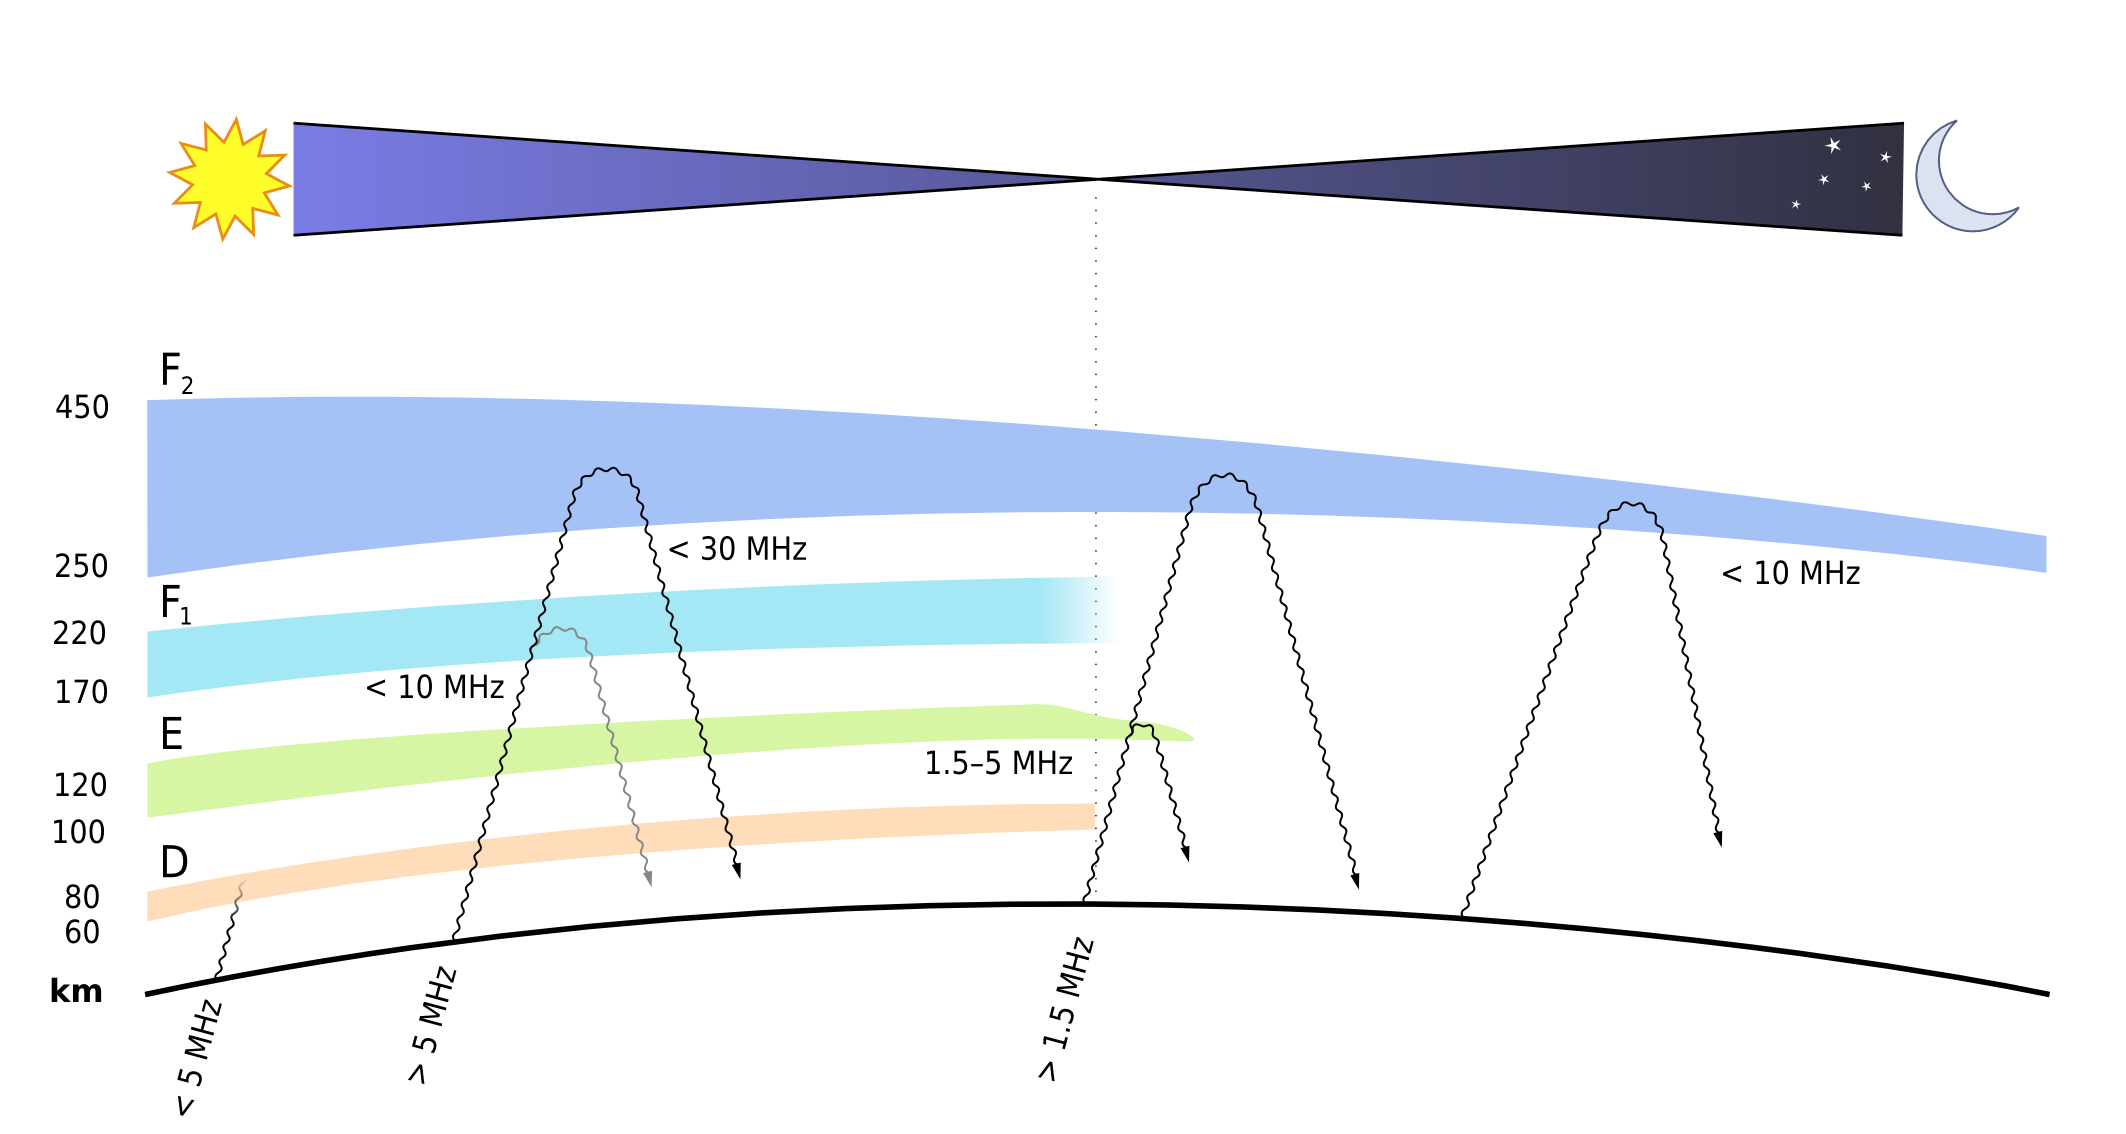
\includegraphics[width=11cm]{./png/Amfu-Ionosphere.png}
 \caption{Aufbau der Ionosphäre und reflektierende Eigenschaften der Schichten}
 \label{fig:ionosphere}
\end{figure}


Insgesamt besteht die Ionosphäre aus drei Schichten, die D-, E- und F-Schichten genannt werden. Die D-Schicht dämpft, die E-Schicht reflektiert tiefere Frequenzen und die F-Schicht höhere. Bei Sonneneinstrahlung (d. h. am Tag) werden Moleküle in der Ionosphäre durch Röntgen- und EUV\footnote{EUV: Extreme ultraviolette Strahlung mit Wellenlängen von 14 bis 80 nm}-Strahlung ionisiert. Eine weitere Rolle spielt die Sonnenfleckenzahl, die sich 2007 in einem Minimum befand und alle 11 Jahre ein Maximum erreicht. Je mehr Sonnenflecken vorhanden sind, desto stärker wird die Ionosphäre bei Sonneneinstrahlung ionisiert. Der Einfluss der Sonnenflecken ist nicht zu vernachlässigen; so sind HF-Frequenzen ab etwa 20 MHz während eines Minimums nicht verwendbar, in einem Maximum jedoch können weltweite Verbindungen beinahe den ganzen Tag entstehen.

\subsection{D-Schicht}
Die unterste der ionisierten Schichten existiert nur am Tag und reflektiert keine Signale. Tiefe Frequenzen unter 5 MHz werden so stark gedämpft, dass das 80-m- und das 160-m-Band nicht mehr benutzbar ist, auf höhere Frequenzen hat es keine grossen Auswirkungen.

Nach Sonnenuntergang verschwindet die D-Schicht sehr schnell, da die Ionen aufgrund der hohen Konzentration schnell wieder rekombinieren.

Bei sehr starker Sonnenaktivität kann der sogenannte \textit{Mögel-Dellinger-Effekt} auftreten. Dann ist die D-Schicht so stark ionisiert, dass das gesamte HF-Band für einige Minuten bis Stunden mehr oder weniger tot ist.

\subsection{E-Schicht}
Tagsüber dämpft die E-Schicht Frequenzen über 5 MHz, da die Ionenkonzentration für eine Reflexion zu gering ist. Tiefere Frequenzen werden reflektiert, müssen aber zuerst die D-Schicht passieren. Die Ionisierung befindet sich um die Mittagszeit in einem Maximum und verringert sich danach wieder langsam.

Nach Sonnenuntergang rekombiniert die E-Schicht innerhalb ungefähr einer Stunde nahezu vollständig. Innerhalb dieser Stunde kann sie für kurze Verbindungen über 500 km genutzt werden, da das 80-m- und 160-m-Band dann nicht mehr durch die D-Schicht gesperrt ist.

Im Sommer tritt manchmal manchmal die \textit{Sporadische E-Schicht} ($\textrm E_S$) auf. Es ist nicht klar, wie sie entsteht. An ihr wird sogar VHF reflektiert, was Überreichweiten und hohe Signalstärken ermöglicht. HF wird an einer tieferen Schicht als sonst reflektiert und erlaubt so Verbindungen über kürzere Distanzen von unter 500 km \textit{(Short Skip)}.

\subsection{F-Schicht}
Die F-Schicht ist die wichtigste für HF. Sie besteht am Tag aus zwei verschiedenen Schichten: Der $\mathrm F_1$- und der $\mathrm F_2$-Schicht. In der $\mathrm F_1$-Schicht werden neue Ionen gebildet, die stärkste Ionenkonzentration befindet sich in der $\mathrm F_2$-Schicht. 

Da sich in der Region der $\mathrm F_2$-Schicht nur noch wenige Gasmoleküle befinden, benötigen die Ionen sehr lange zur Rekombination. Sie besteht darum auch während der Nacht, die Stärke nimmt aber ab und somit auch die \link{MUF}.

\section{Arten der Wellenausbreitung}
\subsection{Bodenwelle} \label{sec:bodenwelle}
Die Bodenwelle \textit{(Ground Wave)} hat bei LF eine Reichweite von über 400 km\footnote{Bei gebirgigem Gelände etwa die Hälfte, bei Ozeanen u. ä. mehr als das Zweifache.}, bei HF reicht sie jedoch auf 80 m knapp 150, auf 10 m nur noch um die 30 Kilometer weit. Sie bewegt sich in der Troposphäre über dem Boden und wird hauptsächlich vom Boden gedämpft. Dabei wirken sich zum Beispiel dichte Vegetation (Wald), trockener Boden und stark bebaute Gebiete negativ auf die Reichweite aus, was aber zum Beispiel bei militärischen Einsätzen gewünscht sein kann. Gut leitende Untergrunde wie Wasser führen zu grösseren Reichweiten.

\subsection{Raumwelle}\label{sec:raumwelle}
Mit der Raumwelle \textit{(Sky Wave)}, die wie die Bodenwelle von jeder HF-Antenne erzeugt wird, ist es möglich, durch (Mehrfach-)Reflexionen an der Ionosphäre grössere Distanzen zu überbrücken. Pro Hop (Reflexion auf der Erde) können mehrere hundert Kilometer zurückgelegt werden, sogar bei Nacht noch über 500. Bei jeder Reflexion wird das Signal gedämpft.

Je flacher der Abstrahlwinkel der Antenne ist, desto höhere Frequenzen kann man verwenden und desto weiter kommt man mit einem Hop. Umgekehrt sollte für eine Nahverbindung eine tiefe Frequenz und ein steiler Abstrahlwinkel über 30° gewählt werden.

Für Verbindungen über weite Entfernungen eignen sich die Stunden um Sonnenauf- und -untergang am besten, da zu dieser Zeit die F-Schicht zwischen den Stationen gut aufgebaut ist. Beispiel: Bei Verbindungen in die USA gegen den Mittag wäre dort Nacht und die F-Schicht sehr dünn, so dass diese Frequenzen nicht reflektiert würden. Um Sonnenuntergang wird die F-Schicht hier langsam abgebaut, über dem Atlantik ist sie am stärksten, und in den USA wird sie gerade aufgebaut.

Die Raumwelle wird ab VHF zur Space Wave.

\subsection{Space Wave}
Die \textit{Space Wave} tritt ab VHF aufwärts auf. Sie bewegt sich quasi-optisch, also ungefähr bis zum Horizont, da sie kaum gebeugt wird und dann im All verloren geht. Allerdings wird sie zum Beispiel an Bergen reflektiert und von Wäldern und Häusern gedämpft, wodurch ihre Reichweite um einiges eingeschränkt wird. 

\section{QRN – Störungen in der Atmosphäre}
Vor allem unterhalb des 20-m-Bandes können atmosphärische Störungen eine solche Stärke erreichen, dass Gegenstationen trotz hoher Signalstärke nur noch schlecht hörbar sind. Im Sommer nimmt das QRN aufgrund häufigerer Blitzentladungen zu.

\subsection{Blitze}\label{sec:blitze}
Während der Entladung eines Blitzes entsteht ein elektromagnetischer Puls, da sich während einer kurzen Zeit extreme Spannungsänderungen vollziehen und gewaltige Ströme fliessen. Solche Störungen lassen sich in sehr weiter Distanz noch messen. Mit speziellen Systemen ist es sogar möglich, die Blitze zu orten. So können ungefähr 95\,\% der Blitze festgehalten werden.

Die von Blitzen erzeugten Signale werden \textit{Spherics}, \textit{Tweeks} oder \textit{Whistler} genannt, je nachdem, wie weit sie «gereist» sind. Spherics erzeugen im Wasserfalldiagramm nur Striche, Tweeks leicht gebogene Striche und Whistler hinterlassen Kurven, da Frequenzen höherer Wellenlänge schneller sind und so früher ankommen. Tweeks und Whistler sind als Pfeifton hörbar, dessen Frequenz sich ändert. Bei Tweeks dauert dies ein paar Hundertstelssekunden, Whistler wandern entlang des Erdmagnetfeldes und sind aufgrund der noch grösseren zurückgelegten Distanz länger hörbar – bis mehrere Sekunden lang. Sferics sind als kurzes Knacken hörbar.

\begin{figure}[h!]
 \centering
 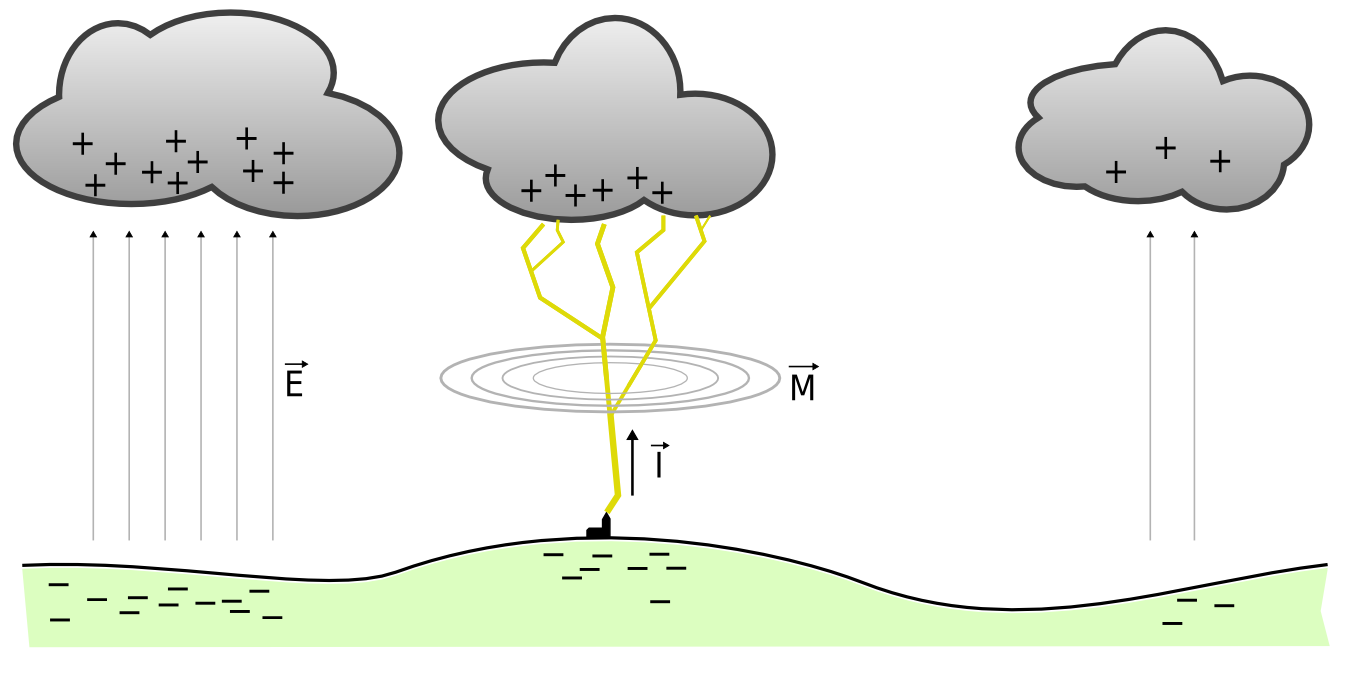
\includegraphics[width=11cm]{./png/Amfu-Blitz.png}
 \caption{Entladung eines Blitzes: Bei einem Gewitter besteht durch den Ladungsunterschied zwischen Wolke und Erde ein elektrisches Feld. Bei einem Blitz fliessen Elektronen (d. h. ein starker Strom) zur hier positiv geladenen Wolke, dadurch entsteht kurzfristig ein starkes magnetisches Feld.}
 \label{fig:blitz}
\end{figure}


Entladungen, die sich in der Nähe ereignen, erzeugen Störungen über das ganze Spektrum, hörbar in den unteren Bändern als starkes Knacken, in den oberen als kurz stark erhöhtes Rauschen.

\begin{figure}[h!]
 \centering
 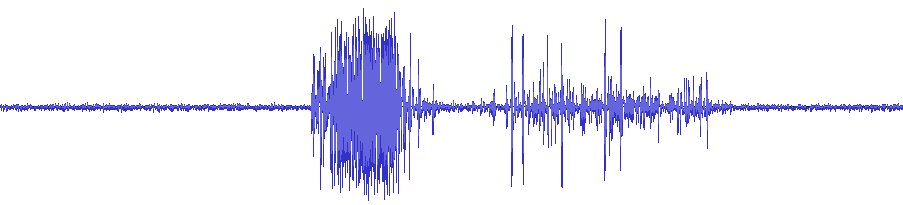
\includegraphics[width=5cm]{./png/Blitz-20M.png}
 \caption{Störung durch einen Blitz auf 21 MHz (Dauer des Ausschnittes: 2 Sekunden)}
 \label{fig:flash20}
\end{figure}


\section{QRM – Von Menschen verursachte Störungen}
QRM kann viele Ursachen haben. Auf Bändern mit hohem Funkverkehr können es ganz einfach andere Stationen sein, die so weit entfernt sind, dass sie nicht mehr verstanden, aber dennoch empfangen werden können und so den eigenen Funkverkehr stören. 

Eine andere häufige Störungsursache sind elektrische Geräte wie Computer, die in der Nähe laufen.





\chapter{Modulation}
\lit{«Modulationsverfahren zur Sprachübertragung» von Florian B. Wörter (\href{http://www.woerter.at/dud/stuff/modulationsverfahren.pdf}{PDF})}
\lit{Formeln zu AM, FM und PM: Formelsammlung}
Ganz am Anfang hat man grundsätzlich ein Signal im Basisband. Das kann sowohl ein Sprach- als auch ein digitales Signal sein, mit Frequenzen zwischen 0 und 30 kHz (für Satelliten werden noch höhere verwendet, bei der Sprachübertragung geht man im Amateurfunk meist nur bis 3 kHz). In den folgenden Grafiken wird ein Sprachsignal amplitudenmoduliert.

Das Sprachsignal befindet sich zunächst im Basisband stellt das USB dar. Das LSB existiert noch nicht, da es negative Frequenzen in der Praxis nicht gibt.

\begin{figure}[h<!]
 \centering
 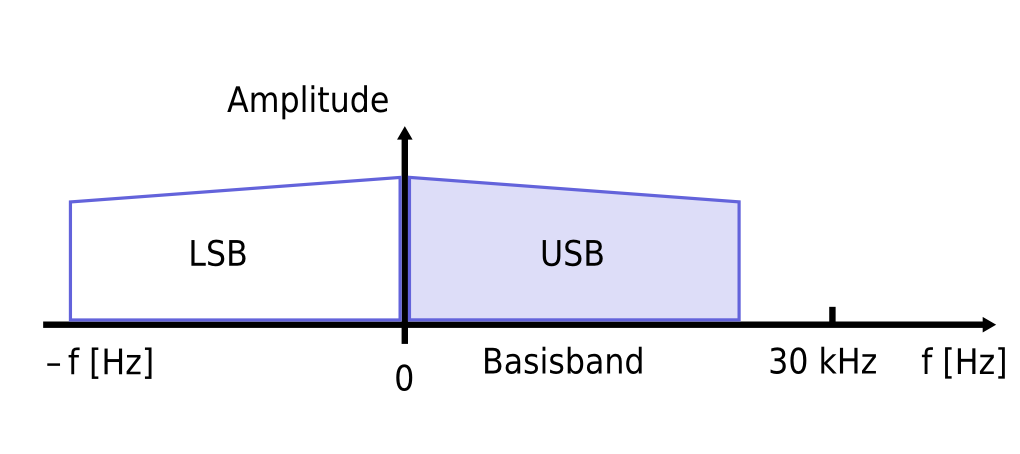
\includegraphics[width=8cm]{./png/Amfu-Modulation-Basisband.png}
 \label{fig:basisband}
\end{figure}


Nun nimmt man eine hochfrequente Trägerschwingung zur Hilfe. Das Signal wird auf sie aufgeprägt (zum Beispiel amplitudenmoduliert), indem man gewisse Eigenschaften (je nachdem die Amplitude, Frequenz oder Phase) der Trägerschwingung proportional zum Signal verändert. So wird das Basisband in den gewünschten Hochfrequenzkanal verschoben.

\begin{figure}[h!]
 \centering
 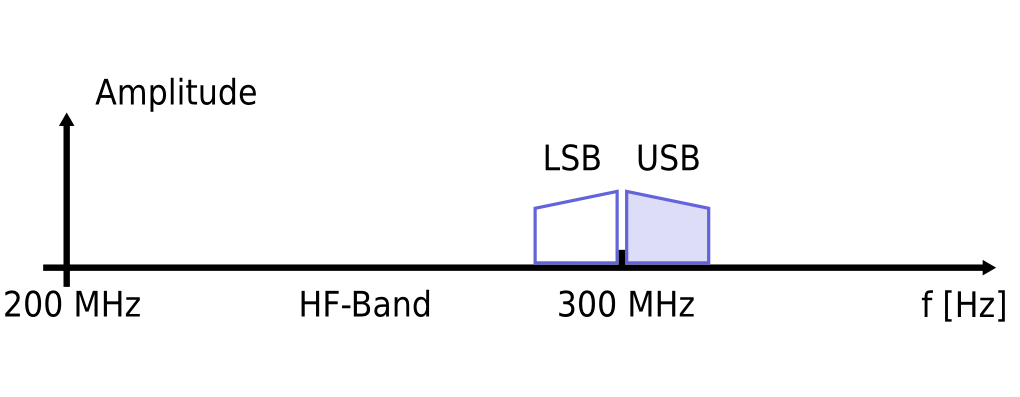
\includegraphics[width=8cm]{./png/Amfu-Modulation-HF.png}
 \label{fig:hfband}
\end{figure}


Während der Amplitudenmodulation wird noch das LSB erzeugt, und es entsteht das Doppelseitenband, das die zweifache NF-Bandbreite aufweist. Da das LSB eine Spiegelung ist, ist es jedoch unnötig und wird etwa bei SSB herausgefiltert.

Man unterscheidet zwischen analogen und digitalen Signalen. Digitale Signale sind zeitdiskret, es wird zwischen festgelegten Zuständen (wie 0/1) gewechselt. Analoge Signale sind zeitkontinuierlich. 

\section{Analoge Modulation}

\subsection{AM}
Bei der Amplitudenmodulation wird auf die Amplitude eingewirkt. Im Frequenzsprektrum wird der Träger als Peak und die beiden Seitenbänder – die die selben Informationen enthalten – sichtbar. Auf dem Träger liegt der grösste Teil der Leistung. Der maximale Wirkungsgrad beträgt (bei einem Modulationsgrad von 1) 17 \%.

\begin{figure}[h!]
 \centering
 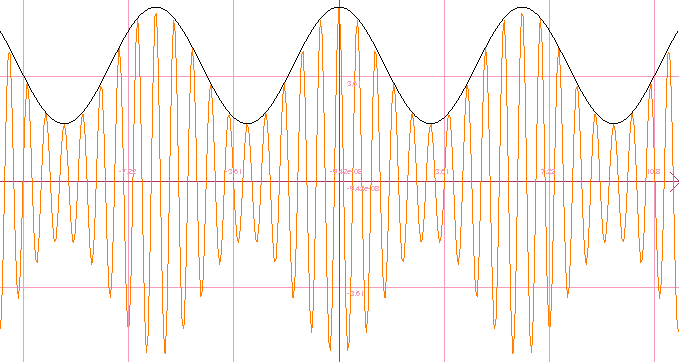
\includegraphics[width=8cm]{./png/Graph_AM.png}
 \caption{Amplitudenmodulation, vereinfacht dargestellt. Das (verschobene) Signal ist schwarz, der Träger orange dargestellt.}
 \label{fig:am}
\end{figure}

Der Modulationsgrad eines AM-Signals ist definiert als das Verhältnis der Amplitude des Signals zur Amplitude des Trägers:

\[
 m = \frac{S_M}{S_T}
\]


Ist der Modulationsgrad grösser als eins, wird das Signal übermoduliert und es treten Verzerrungen auf. 

AM wird von den meisten Rundfunksendern im HF-Band verwendet.

\begin{figure}[h!]
 \centering
 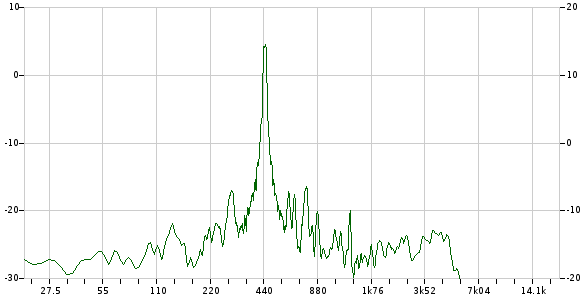
\includegraphics[width=8cm]{./png/AM-Analysis.png}
 \caption{AM-Signal mit dem typischen Peak des Trägersignals}
 \label{fig:amAnalysis}
\end{figure}

Die meisten modernen Amateurfunkgeräte bieten immer noch die Amplitudenmodulation an. Die Aufbereitung der AM geschieht jedoch schon in den Vorstufen des Sendeteils, daher ist die Leistung in der Regel auf 25 \% gegenüber LSB/USB reduziert, um die Endstufe nicht zu überlasten und auch die Linearität zu gewährleisten.

In «echten» AM-Sendern wurde die Modulation bei der Endstufe selbst vorgenommen, und diese konnte im C-Betrieb mit wesentlich grösserer Leistung arbeiten. Dieser scheinbare Vorteil ändert aber nichts an der schlechten Energieeffizienz von AM gegenüber SSB.

AM wird im Amateurfunk kaum noch verwendet. Es gibt noch einige AM-Runden im 80m-Band von OMs, die alte Geräte restaurieren und auch betreiben. Auch im 10m-Band bei 29 MHz sind meist amerikanische OMs in AM aktiv (dort spricht man von «Wintage-Radios»).

Im kommerziellen und auch militärischen Flugfunkverkehr im VHF- und UHF-Bereich wird nach wie vor AM verwendet. Der Grund dafür ist vor allem die Beibehaltung einer Kompatibilität mit älteren Ausrüstungen. Ein weiterer Grund ist die Gewährleistung der Verständlichkeit, wenn z. B. zwei Benutzer gleichzeitig sprechen; dies würde mit FM nicht so sein und könnte zu fatalen Missverständnissen führen. Auf Kurzwelle wir der Flugfunk in USB betrieben, allerdings in einem festen Kanalraster in kHz-Schritten.

Im CB-Funk wurde lange Zeit nur AM gesendet und das Kanalraster entsprechend in 10-kHz-Schritten ausgelegt. Heute wird da vorwiegend in FM im gleichen Kanalraster gearbeitet, oder aber auch in SSB mit Umschaltung LSB/USB. Im «illegalen» CB-Bereich oberhalb 27 405 kHz wird vorwiegend in USB mit 5-kHz-Raster gearbeitet.

\subsection{FM}
Bei der Frequenzmodulation wird auf die Frequenz eingewirkt. Hier wird die Frequenz selber moduliert, was das Signal relativ unanfällig gegenüber Störungen der Amplitude (wie kurze Signalstärkenschwankungen) macht. Mit FM werden die meisten heutigen Radiosendungen moduliert, wie auch Funk auf VHF/UHF.

\begin{figure}[h!]
 \centering
 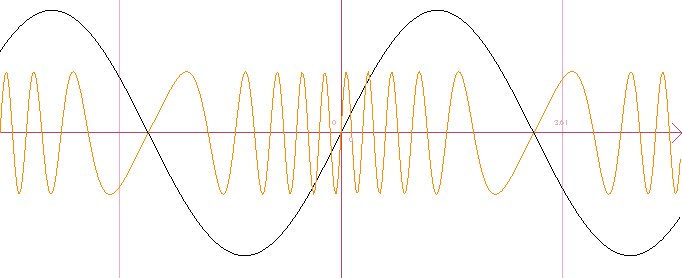
\includegraphics[width=8cm]{./png/Graph_FM.png}
 \caption{Vereinfachte Darstellung von Frequenzmodulation. Das Signal ist schwarz, der Träger orange dargestellt}
 \label{fig:fm}
\end{figure}

Bei FM gewinnt immer das stärkere Signal, d. h. wenn zwei Stationen auf der selben Frequenz senden, hört man den schwächeren nicht. Bei ähnlicher Signalstärke stören sie sich gegenseitig, und man versteht gar nichts. Deshalb wird im Flugfunk auch immer noch AM verwendet.

\begin{figure}[h!]
 \centering
 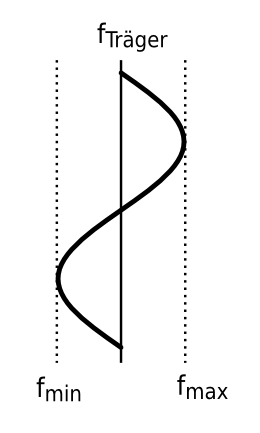
\includegraphics[width=3cm]{./png/Amfu-FM-Wasserfall.png}
 \caption{Sinusförmiges Signal, dieses Mal in der Wasserfalldarstellung. Hier wird die ursprüngliche Signalform wieder sichtbar.}
 \label{fig:fmWaterfall}
\end{figure}

Auf HF kann man mit modernen Transceivern zwar FM senden, was prinzipiell nach dem FMG auch erlaubt wäre. In den Bandplänen, die von den Amateuren selbst ausgearbeitet wurden, ist das jedoch nicht vorgesehen. Einzig im 10m-Band oberhalb etwa 29.5 MHz wird exklusiv in FM gearbeitet, und es gibt dort auch Relais-Stationen mit 100 kHz Abstand zwischen RX und TX (z. B. Relais hb9hd auf 29 660 kHz TX bzw. 29 560 kHz RX).

\subsection{SSB}
Single Side Band; hier wird nur das untere (Lower Side Band, LSB) bzw. das obere Seitenband (Upper Side Band, USB) verwendet, was mit 2.7 kHz (\link{NF-Bandbreite}) weniger als der Hälfte der von AM benötigten Bandbreite entspricht. Da zudem auch der Träger herausgefiltert wird, benötigt man so nur einen Sechstel der Leistung, die für AM notwendig wäre.

Unterhalb von 10 MHz wird meist LSB verwendet, darüber USB.

SSB findet bevorzugt auf dem HF-Frequenzband Verwendung.

\section{Digitale Modulation}
Seit einigen Jahren wird auch für Sprechfunk vermehrt digitale Modulation (vor allem QPSK) erprobt und auch angewendet. Hier wird das analoge Sprachsignal abgetastet und so digital codiert. Danach steht ein digitaler Datenstrom zur Verfügung. Dies ermöglicht auch weltweites Routing übers Internet. Es scheint, dass sich der D-Star-Standard von Icom diesbezüglich durchsetzt.

Heute dominieren sogenannte OFDM-Verfahren, wo innerhalb eines Kanals eine Vielzahl von PSK-, QPSK- oder QAM-modulierte Träger übertragen werden, auf denen dann die erforderlichen Biströme verteilt sind. Ein Beispiel ist DRM auf KW/MW-Rundfunk. 

Die Vorteile sind eine klare Modulation wie in FM, eine relative Unempfindlichkeit gegen Verzerrungen durch die Ionosphäre und ein sauberes Spektrum. Es ist damit auch möglich, Standbilder oder grössere Datenmengen zu übertragen. Diese Verfahren werden durch einen PC oder von Standalone-Geräten (z. B. von AOR), die an die Mike- und NF-Buchsen angeschlossen werden, erzeugt und demoduliert.

\subsection{ASK}
Das \textit{Amplitude Shift Keying} (Amplitudenumtastung) wird für digitale Übertragungen nur noch selten verwendet. Der Nachteil bei ASK ist die unsichere Übertragung bei schlechten Verhältnissen, da eine kleinere Amplitude und ein plötzlich schwächer ankommendes Signal schwer zu unterscheiden sind. 

Die einfachste Art von ASK ist das \textit{On-Off Keying} (OOK), das unter anderem von LF-Zeitzeichensendern wie HBG auf 75 kHz eingesetzt wird.

\subsection{FSK, AFSK, MFSK}
\textit{Frequency Shift Keying} (Frequenzumtastung) ist «digitale» Frequenzmodulation. Bei FSK wird direkt die Frequenz des HF-Signals verändert, bei AFSK wird das Audiosignal umgetastet und auf HF aufmoduliert. In der Wasserfalldarstellung ergibt sich so ein Bild wie in \link{Grafik 12 (RTTY-Wasserfall)}.

\begin{figure}[h!]
 \centering
 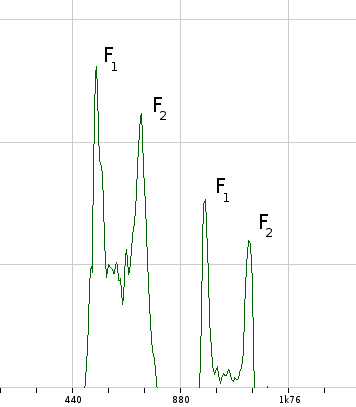
\includegraphics[width=4cm]{./png/FSK-Analysis.png}
 \caption{Zwei schmalbandige FSK-Signale, Spektrumanalyse}
 \label{fig:fsk}
\end{figure}

Bei MFSK \textit{(Multiple Frequency Shift Keying)} wird zwischen mehreren verschiedenen Frequenzen umgetastet. MFSK wird zum Beispiel bei Olivia benutzt.

\begin{figure}[h!]
 \centering
 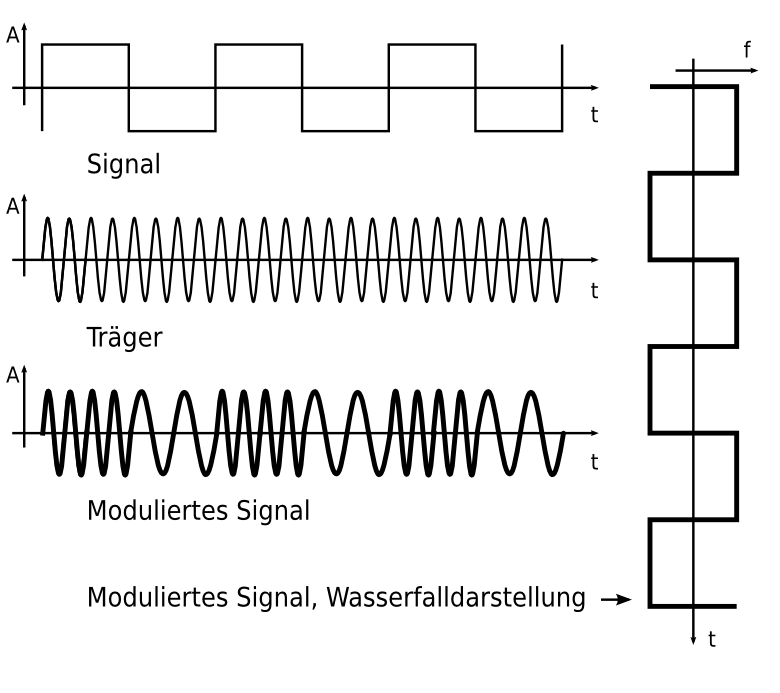
\includegraphics[width=8cm]{./png/Amfu-FSK.png}
 \caption{Modulation eines digitalen Signals (0 und 1). Die Amplitude wird im Wasserfalldiagramm wieder sichtbar.}
 \label{fig:fskMod}
\end{figure}


\subsection{PM}
Bei der Phasenmodulation wird auf die Phase eingewirkt. Eine vereinfachte Form ist das Binary Phase Shift Keying (BPSK), bei dem zwischen zwei Zuständen (0 und 1) gewechselt wird. Beim Wechsel wird die Phase um 180° gedreht, d. h. die Sinuskurve wird um eine halbe Schwingung ($\pi$) verschoben. Phasenmodulation wird für analoge Übertragungen kaum eingesetzt, eignet sich für Digitales sehr gut.

\begin{figure}[h!]
 \centering
 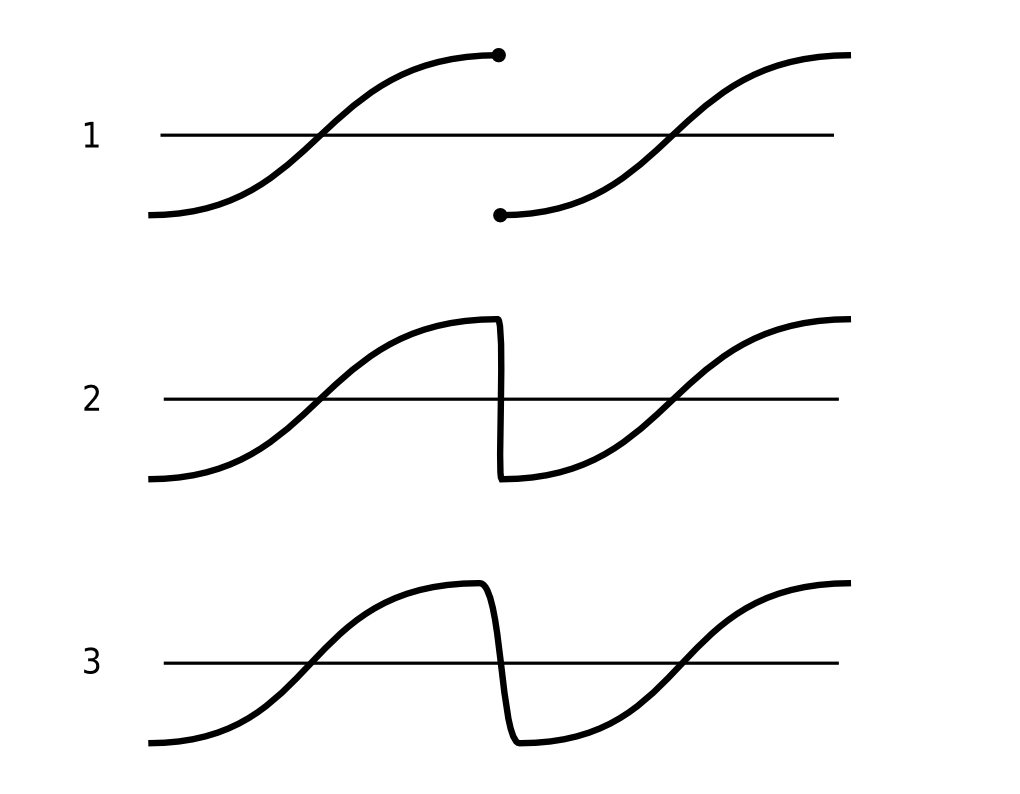
\includegraphics[width=6cm]{./png/Amfu-PM.png}
 \caption{Phasenmodulation: Phasenwechsel um 180°}
 \label{fig:pm}
\end{figure}

\begin{figure}[h!]
 \centering
 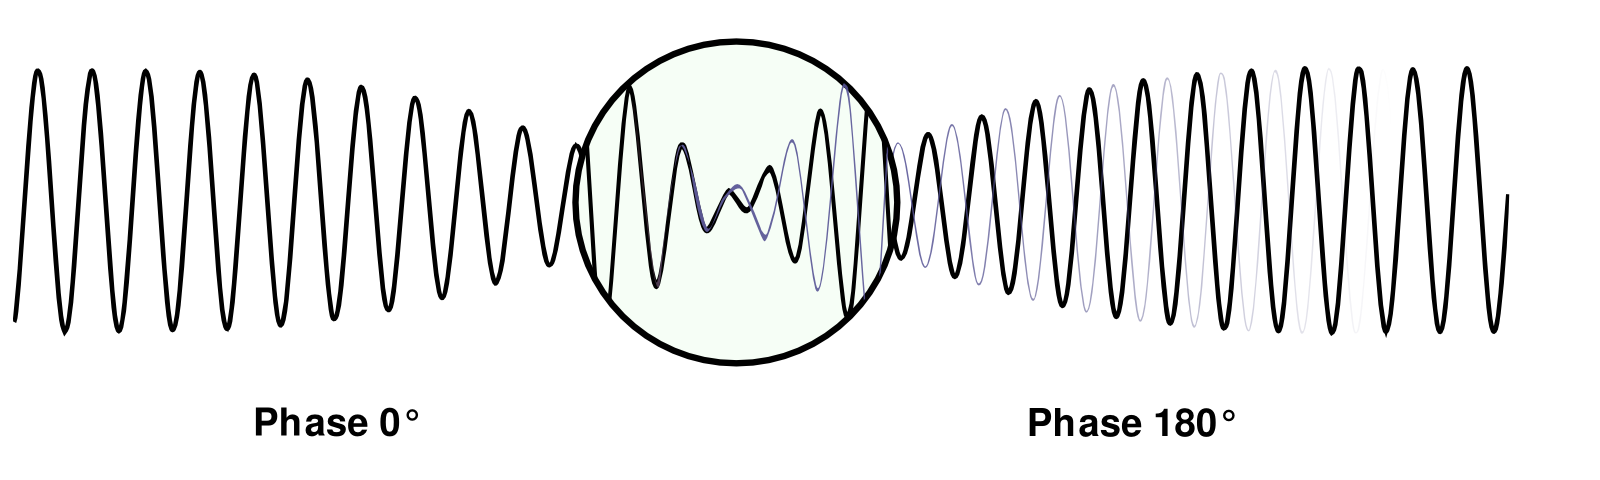
\includegraphics[width=10cm]{./png/Amfu-PSK.png}
 \caption{PSK: Die Phase wird um 180° gedreht}
 \label{fig:psk}
\end{figure}

Beim Phasenwechsel (in \link{Grafik 10 oben} um 180°) entsteht während dem Phasenwechsel für kurze Zeit eine höhere Frequenz (und somit eine höhere Bandbreite), da die beiden Punkte verbunden werden müssen (1). Eine senkrechte Verbindung würde aber zu einer sehr hohen Frequenz führen (2). Möglich wäre zum Beispiel die Kurve 3, die sich durch den Widerstand von Kabel etc. (steigt mit höherer Frequenz) automatisch ergibt. Bei PSK31 wird das Signal beim Übergang zusätzlich noch abgeschwächt.

\chapter{Übertragungsverfahren}\label{sec:uebertr}

Heute existieren hunderte verschiedener Übertragungserfahren. Hier ein kleiner Ausschnitt davon:

\section{CW}
CW (A1A) steht für \textit{Continuous Wave} und wird im Amateurfunk als Synonym für Morsecode verwendet. Die Informationen werden nicht durch das Signal an sich, sondern durch Rhythmus und Pausen übertragen. Da nur ein Trägersignal verwendet wird, ist die Bandbreite mit etwa 300 Hz relativ gering. So sind DX-Verbindungen auf andere Kontinente bei guten Ausbreitungsbedingungen mit wenigen mW möglich.

Die häufiger verwendeten Zeichen sind kürzer, damit die Übertragung effizienter ausfällt. Daneben existieren viele internationale und lokale Abkürzungen.

\textit{Angabe:} Frequenz

\section{RTTY}
\begin{wrapfigure}{R}{4cm}
%%%%%%%%%%%%%%%%%%%%%%%%%%%%%%%%%%%%%%%%%%%%%%%%%%%%%%%%%%%%%%%%%%%%%%%%%%%%%%%%%%%%%%%
%%% You will need to add \usepackage{wrapfig} to your preamble to use textwrapping %%%
%%%%%%%%%%%%%%%%%%%%%%%%%%%%%%%%%%%%%%%%%%%%%%%%%%%%%%%%%%%%%%%%%%%%%%%%%%%%%%%%%%%%%%%
 \centering
 
\includegraphics[height=4cm]{png/RTTY-BaudlineSmall.png}
 % RTTY-BaudlineSmall.png: 47x163 pixel, 72dpi, 1.66x5.75 cm, bb=0 0 47 163
 \caption{RTTY-Wasserfall}
 \label{fig:rttyWaterfall}
\end{wrapfigure}

Radio Teletype war vor PSK31 das am meisten verwendete digitale Übertragungsverfahren unter Amateurfunkern, da sie einfach zu Übermitteln und zu decodieren ist. Ein durch \plink{sec:fsk}{FSK} bzw. AFSK bedingter Nachteil ist die Bandbreite von mehreren 100 Hz: Sie benötigt mehr Leistung und belegt einen grösseren Teil des Frequenzbandes als andere digitale Verfahren. Die Zeichen werden mit dem Baudot-Code codiert. Er wurde von Èmile Baudot für ein Telegrafengerät entwickelt, das mit fünf Fingern bedient werden kann. Einzelne Zeichen haben immer eine Länge von 5 Bit, womit 32 verschiedene Zeichen möglich sind. Da dies für das Alphabet zu wenige sind, wird ein Umschaltcode verwendet, der zwischen der Buchstaben- und der Zahlentabelle wechselt. Geht dieser bei der Übertragung verloren, werden falsche Zeichen angezeigt. Es ist ausserdem möglich, mit invertierter Polarisation zu senden, dann sind Mark und Space vertauscht.

Im Amateurfunk verwendet man standardmässig eine Baudrate von 45.45 Bd und kleinen Shifts von etwa 180 Hz. Der Deutsche Wetterdienst sendet mit 50 Bd.

\textit{Angaben:} Mittelfrequenz, Shift, Baudrate, Polarisation

\subsection{PSK31}
Dieses digitale Übertragungsverfahren existiert erst seit wenigen Jahren. Es wurde von Peter Martinez, g3plx, für den Amateurfunk entwickelt. Anders als andere moderne Übertragungsverfahren soll es keine fehlerfreie Übertragung garantieren, da man mit solchen Verfahren bei schlechten Verbindungsverhältnissen statt nur bruchstückhaftem Text schnell gar nichts mehr empfangen kann. In dieser Hinsicht ist ist PSK31 gut mit CW vergleichbar, da auch mit schwierigen Verhältnissen noch Verbindungen zustande gebracht werden können. Mit 50 wpm entspricht die Übertragungsgeschwindigkeit der durchschnittlichen Anschlagsrate bei der Tastatur.

Durch die sehr geringe Bandbreite (etwa 32 Hz, weniger als CW!), die der Übertragungsrate von 31.25 Bits/s entspricht, kann mit kleiner Leistung über weite Distanzen gesendet werden. Ermöglicht wird dies durch die Phasenmodulation.

\begin{figure}[h!]
 \centering
 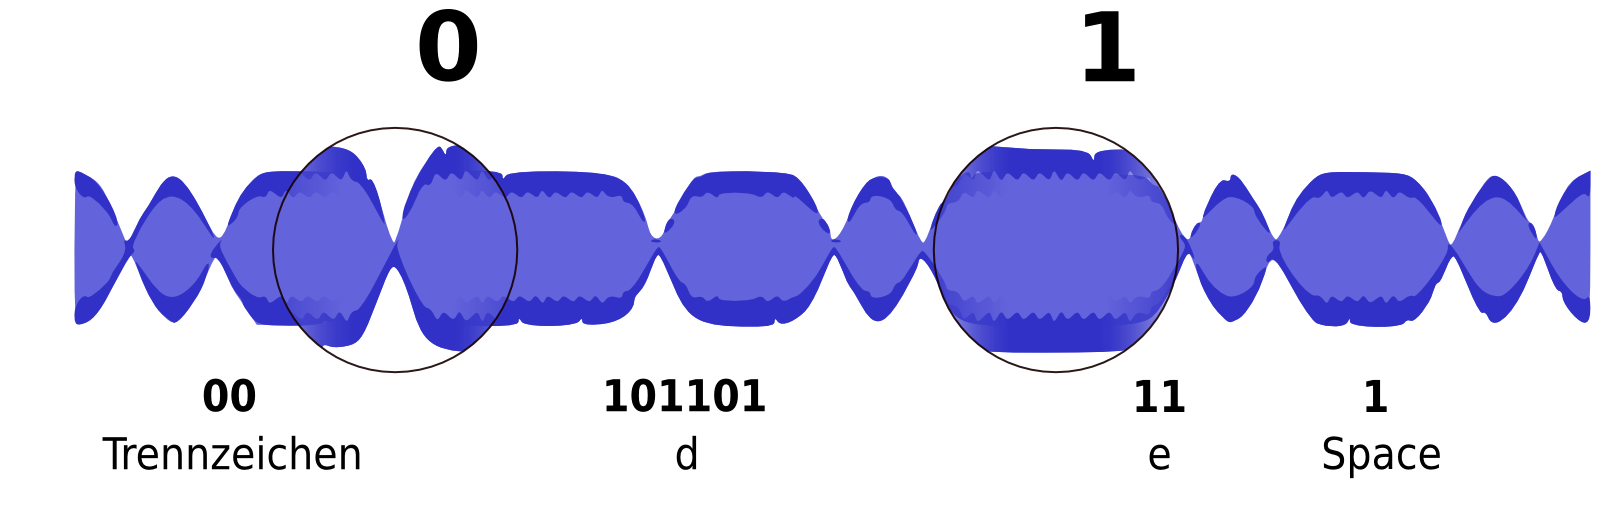
\includegraphics[width=6cm]{./png/Amfu-PSK31-0101.png}
 \caption{Ausschnitt eines PSK31-Datenstroms}
 \label{fig:psk31}
\end{figure}


Die Zeichen werden in Varicode, einer weiteren Entwicklung von g3plx, übermittelt. Sie haben, je nach Häufigkeit (in englischem Text), eine unterschiedliche Länge. Ein Wechsel zwischen zwei Phasen steht für eine 0, eine gleichbleibende Phase für eine 1. Zwei aufeinander folgende Nullen werden als Trennzeichen zwischen zwei Zeichen verwendet.

In Grafik \ref{fig:psk31} wird der Text «de» mit PSK31 übermittelt. Das d wird durch 101101 codiert, das e durch 11. Die folgende 1 ergibt einen Leerschlag.

Die Weiterentwicklung QPSK31 ermöglicht mit Quadratur-Phasenmodulation eine schnellere Übertragung. Das Signal wird dabei um ein Vielfaches von 90 Grad verschoben, was vier mögliche Zustände ergibt. 

\textit{Angabe:} Frequenz

\subsection{Olivia}
Ein neueres MFSK-Verfahren. Die Übertragung ist selbst dann noch möglich, wenn das Signal 10 dB unter dem Rauschpegel liegt. Je nach Anzahl Tönen (2 bis 256) beansprucht diese Übertragungsart eine Bandbreite von 125 bis 2000 Hz.

\subsection{Pactor}
Mit PACTOR, einer Weiterentwicklung der digitalen Betriebsart Amtor, ist es möglich, auch bei schlechten Verhältnissen fehlerfrei Daten zu übertragen, da dann zu robusteren Übertragungsverfahren gewechselt wird. Ausserdem kann man auf Mailboxen zugreifen und so mobil Mails abrufen.

Version I überträgt 100--200\,bits/s, PACTOR-IV bis 5512\,bits/s ohne Kompression. Anders als das offene PACTOR sind PACTOR-II und höher allerdings proprietär, das heisst, die genaue Implementierung ist unbekannt, wodurch Modems nur durch den Entwickler SCS hergestellt werden können (und diese deshalb auch entsprechend teurer sind).

Die Daten werden bei PACTOR mittels \plink{sec:fsk}{FSK} übertragen, bei PACTOR-II und höher mit verschiedenen PSK-Varianten (siehe \plink{sec:pm}{PM}). Bevorzugte Baudraten sind 300 Bd auf HF, 1200 Bd auf VHF/UHF, 9600 Bd auf UHF.

\textit{Angaben:} Frequenz, Baudrate

\subsection{SSTV}
Bei diesem etwas spezielleren computergestützten Verfahren (Slow Scan Television) werden Bilder ausgetauscht. Sie haben üblicherweise 256 Zeilen, dies kann jedoch zwischen den verschiedenen Formaten variieren.

\textit{Angaben:} Frequenz, Format

\subsection{DAB/DRM}
DAB (Digital Audio Broadcasting) und DRM (Digital Radio Mondiale) sind Verfahren zur digitalen Übertragung von Daten (speziell Radiosendungen). Sie basieren beide – wie übrigens auch ADSL – auf OFDM \textit{(Orthogonal Frequency Division Multiplex)}, also der gleichzeitigen Übertragung von mehreren hundert (bei DAB bis 1536) PSK-Strömen. Die Signale sind ungefähr 10 kHz breit bei DRM bzw. etwa 1.5 MHz bei DAB. Neben Ton können über verschiedene Dienste auch andere Daten übertragen werden. Das \textit{MOT} (Multimedia Object Transfer Protocol) etwa ermöglicht die Verteilung von Dateien. So werden parallel zu Radiosendungen komplette Internetseiten mit News übertragen (BWS, Broadcast Webpage System). Per \textit{DLS} (Dynamic Label Service) werden Informationen zur Laufenden Sendung (Name des Stücks, Interpret) übermittelt.

DRM wird auf HF eingesetzt, auf VHF/UHF verwendet man (noch) DAB. DRM+ (DRM für VHF/UHF) hätte hier jedoch einige Vorteile wie bessere Qualität und die Möglichkeit, einzelne Stationen auszusenden; so könnten kleinere Stationen ihre Sendemasten beibehalten.

Nachteilig ist bei Taschenradios der durch die Decodierung bedingte hohe Stromverbrauch.

\subsection{Weitere Übertragungsverfahren}
ATV (Amateur Television), Clover, DATV (Digital Amateur Television), FAX, G-TOR, Hell, JT65, MT63, Packet Radio, SITOR (Simplex Teleprinting Over Radio) 


\chapter{Antennen}\label{sec:antennen}
\lit{Kurzwellen-Drahtantennen Praktikum von Max Rüegger, HB9ACC. Quelle: htc.ch}

\section{Dipol} \label{sec:dipol}
Ein Dipol besteht grundsätzlich aus zwei gestreckten Antennendrähten, die zusammen die Länge $\lambda/2$ (oder ein ganzzahliges Vielfaches davon) ergeben. Sie werden mittig mit hochfrequentem Wechselstrom gespiesen. Der Dipol kann auf der Grundfrequenz und auf ganzzahligen Vielfachen davon betrieben werden.

Neben dem offenen Dipol (Impedanz 50–75 Ohm) existieren noch weitere Varianten wie die \textit{Inverted Vee}, die von einem Antennenmast auf beide Seiten heruntergespannt wird, und verschieden geformte Loops wie der breitbandigere Faltdipol oder der Quad Loop. Loops \textit{(Schleifenantennen)} haben eine höhere Impedanz (240–300 Ohm) und werden aus einem $\lambda$ langen Antennenkabel geformt.

Beim Loop gilt: Je grösser die von der Antenne überdeckte Fläche, desto besser.

\section{Longwire}
Einfache Kabel, die am Ende gespiesen werden (und nicht mittig wie der Dipol). Diese hochomigen Antennen benötigen eine Erdung als Gegengewicht und eine symmetrische Speiseleitung (zum Beispiel eine sogenannte Hühnerleiter). 

\section{Groundplane}
Die Groundplane-Antenne besteht aus einem Strahler und einem Gegengewicht. Der vertikale Strahler wird in Längen von $\lambda/2$, $\lambda/4$ und $\frac{5}{8}\,\lambda$ gebaut. Die $\frac{5}{8}\,\lambda$ eignet sich aufgrund des flacheren Abstrahlwinkels gut für DX-Verbindungen, während die  $\lambda/4$ einen steilen Abstrahlwinkel aufweist.

Als Gegengewicht verwendet man sogenannte Radials (da sie radial von der Antenne weggehen) mit der Länge des Strahlers. Je nachdem werden sie in die Erde vergraben oder über dem Boden gespannt. Werden sie ungefähr einen Meter über dem Boden gehalten, kann der Gewinn unter Umständen um 3 S-Stufen steigen.

Die Impedanz beträgt 36 Ohm, kann aber mit den Radials verändert werden (etwa auf 50 Ohm).

Für mobile VHF/UHF-Antennen kann z.\,B. das Auto als Gegengewicht verwendet werden.

\section{Logper}
Da sie sich auf verschiedenen Bändern einsetzen lassen, wird die Logper-Antenne (auch LPDA, Logarithmic-Periodic Dipole Array, genannt) immer beliebter. Sie ist aus unterschiedlich grossen, gegengleich verdrahteten Dipolen aufgebaut. Beim Senden sucht sich jede Frequenz den passenden Dipol; das vordere Element wirkt als Direktor und das hintere als Reflektor. So sind immer ungefähr drei bis vier Elemente aktiv. Eine Logper ist somit aus der Sicht einer Frequenz eine Dreielement-Antenne und weist auch einen ähnlichen Gewinn auf.

\begin{figure}[h!]
 \centering
 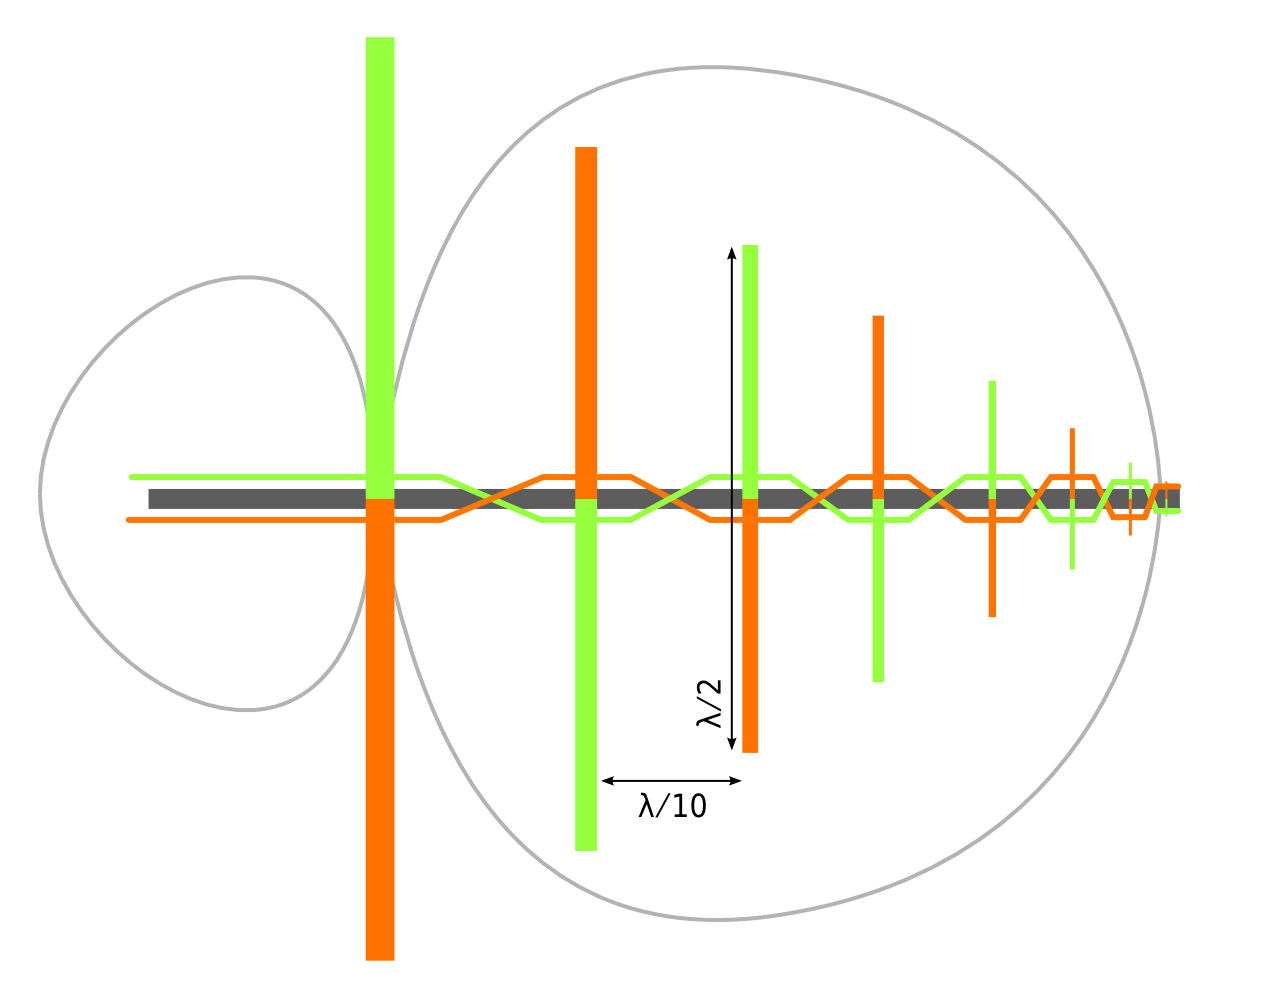
\includegraphics[width=6cm]{./png/Amfu-Logper.png}
 \caption{Aufbau, Stromverteilung und Abstrahldiagramm einer Logper.}
 \label{fig:logper}
\end{figure}

Für einen besseren Gewinn oder eine grössere Bandbreite muss die Logper länger sein. Aufgrund der Grösse wird sie im Amateurfunk praktisch nur für VHF/UHF eingesetzt, bei militärischen Einrichtungen sind auch Logper-Antennen für HF zu sehen.

\section{Yagi} \label{sec:yagi}
Yagis (eigentlich Yagi-Uda-Array; erfunden wurde sie vom Japaner Uda, Yagi übersetzte den Artikel nur zuerst nach Englisch) oder \textit{Beams} werden vor allem im Bereich VHF/UHF verwendet. Sie sind eher schmalbandige Richtstrahlantennen und bestehen aus einem Strahler – ein einfacher Dipol –, einem Reflektor und aus mindestens einem Direktor. Die Direktoren, die in die gewünschte Abstrahlrichtung zeigen, sind etwa $0.05 \lambda$ kürzer, der Reflektor auf der anderen Seite ungefähr $0.05 \lambda$ länger. Ein dreielementiges Yagi hat einen Gewinn von etwa 5 dB, mit weiteren Elementen sind bis 20 dB erreichbar.

\begin{figure}[h!]
 \centering
 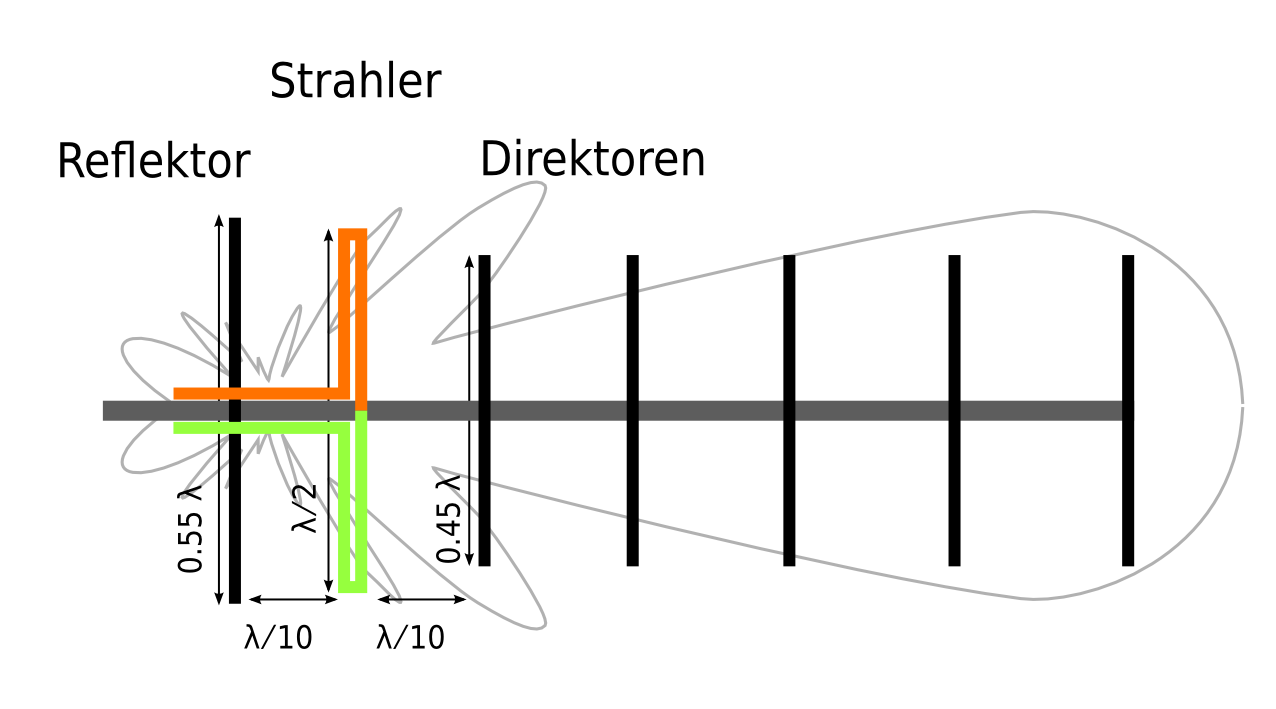
\includegraphics[width=6cm]{./png/Amfu-Yagi.png}
 \caption{Aufbau, Stromverteilung und Strahlungsdiagramm einer Yagi.}
 \label{fig:yagi}
\end{figure}

Auf älteren Hausdächern sieht man teilweise noch Yagis für den Fernsehempfang.

Mit Yagis kann man aufgrund der Richtwirkung in eine bestimmte Richtung besser senden und empfangen. 

\section{Magnetantenne}
Anders als herkömmliche Antennen arbeitet die Magnetantenne mit dem magnetischen Anteil des elektromagnetischen Signals. Sie lässt sich mit Durchmessern um einen Meter sehr platzsparend bauen und eignet sich daher gut für dicht besiedelte Gebiete. Ein Nachteil ist jedoch, dass sie sehr schmalbandig ist und sogar bei Frequenzwechseln innerhalb eines Bandes nachgestellt werden muss.

Ab einem Umfang von mehr als $\lambda∕10$ spricht man wieder von einer elektromagnetischen Antenne, da der elektrische Teil dann wieder zunimmt.

\section{Antennenkabel}
\subsection{Dämpfung}
Dämpfung tritt sowohl im Kabel als auch bei Steckverbindungen auf. Der Verlust bei gecrimpten (geklemmten) Verbindungen ist etwas geringer als bei gelöteten.

\subsection{Koaxialkabel}\label{koax}
Koaxialkabel, oder kurz Koaxkabel, ist aufgebaut aus einem meist kupfernen Innenleiter, der von einem Aussenleiter umgeben ist; beide werden durch ein Dielektrikum getrennt. Der Wellenwiderstand der Leitung hängt vom Verhältnis der Leiterdurchmesser $\frac{D}{d}$ und der Permittivität $\epsilon_r$ des Dielektrikas ab.

\begin{figure}[h!]
 \centering
 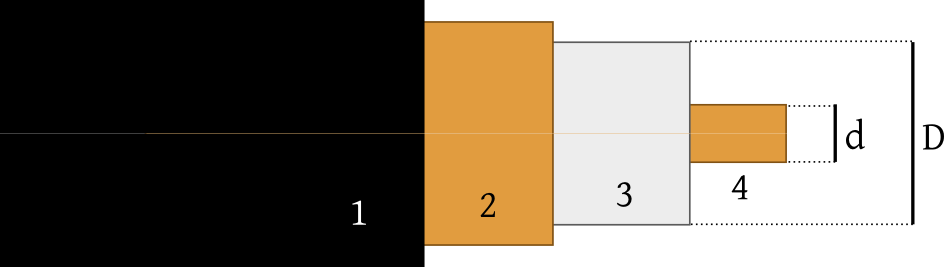
\includegraphics[width=6cm]{./png/Koax.png}
 % Koax.png: 944x267 pixel, 300dpi, 7.98x2.26 cm, bb=0 0 226 64
 \caption{Aufbau von Koaxialkabel. \textbf{1:} Isolation. \textbf{2:} Aussenleiter (Abschirmung). \textbf{3:} Dielektrikum (Isolator). \textbf{4:} Innenleiter (Seele). \imgsrc{Simon A. Eugster, 2013. GFDL 1.3, cc-by-sa 3.0}}
 \label{fig:coax}
\end{figure}

Auch die Ausbreitungsgeschwindigkeit im Koaxialkabel ist von $\epsilon_r$ abhängig, sie beträgt:

\[v = \epsilon_r^{-\frac{1}{2}} c\]

Mit steigendem Aussendurchmesser $D$ sinkt die Dämpfung.


In der folgenden Tabelle ist zu häufigen Kabeltypen der Wellenwiderstand $Z_W$ und der Verkürzungsfaktor $k_v$ angegeben.

\vspace{1em}
\begin{tabular}{lll rr}
\bfseries Kabeltyp & \boldmath $Z_W$ & \boldmath $k_v$ & \multicolumn{2}{c}{\bfseries Dämpfung pro 100 m} \\
                   &                            &                             & \small 10 MHz & \small 100 MHz \\
\toprule \arrayrulecolor{rowsep}
RG-8/U   & $50~\Omega$ &      & 1.8\,dB & 6.7\,dB \\ \midrule
RG-58    & $50~\Omega$ & 0.66 & 4.1\,dB & 15.0\,dB \\ \midrule
RG-59    & $75~\Omega$ & 0.66 & 3.6\,dB & 11.2\,dB \\ \midrule
RG-213/U & $50~\Omega$ & 0.66 & 1.8\,dB & 6.7\,dB  \\ \midrule
\end{tabular}
\vspace{1em}


\subsection{Bandleitung}
Die Bandleitung (auch als \textit{Hühnerleiter} bekannt) dient zum Anschluss von symmetrischen Antennen wie Dipolen und Yagis. Sie besteht aus zwei eifachen Leitern mit Durchmesser $d$, die durch ein Isolationsmaterial mit Permittivität $\epsilon_r$ in einem konstanten Abstand $a$ parallel zueinander geführt werden. Der Vorteil hiervon ist, dass bei symmetrischen Antennen keine Impedanzanpassung notwendig ist, falls die Funkstation symmetrische Kabel unterstützt. Beim Übergang von Koaxkabel zu Bandleitung wird ein Balun benötigt.

\begin{figure}[h!]
 \centering
 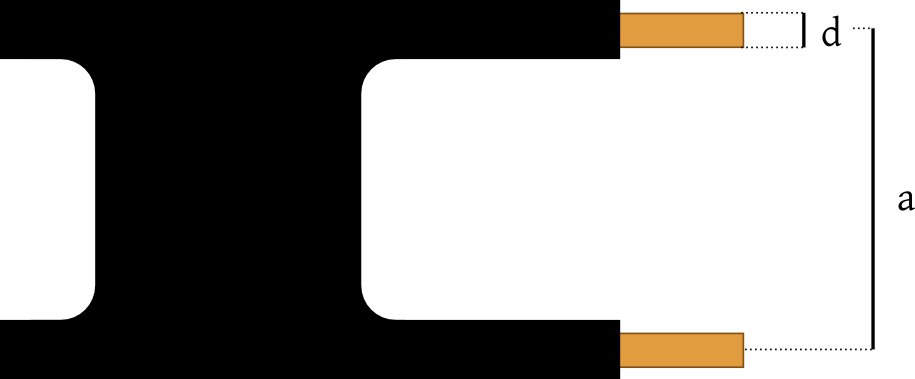
\includegraphics[width=6cm]{./png/Bandleitung.png}
 % Bandleitung.png: 915x379 pixel, 300dpi, 7.75x3.21 cm, bb=0 0 220 91
 \caption{\textbf{d:} Leiterdurchmesser. \textbf{a:} Abstand.}
 \label{fig:bandleitung}
\end{figure}


Der Wellenwiderstand berechnet sich mit:

\[Z_W = \frac{120~\Omega}{\sqrt{\epsilon_r}}\, \mathrm{acosh} \left ( \frac{a}{d} \right ) \]

und ist häufig $450~\Omega$ oder $600~\Omega$.





\chapter{Rufzeichen}\label{sec:rufzeichen}

\section{Schweizer Rufzeichen HBn und HEn}
\begin{tabular}{l p{9cm}}
\bfseries Rufzeichen & \bfseries Verwendung \\ \toprule \arrayrulecolor{rowsep}
HB9 & Normales Präfix für lizenzierte Amateurfunker in der Schweiz. \\ \midrule
HB9x(x) & \textit{Oldtimer} der 60er-Jahre (z. B. Rudolf Stuber mit HB9T) oder \textit{Klubstationen}. \\ \midrule
HB0 & Amateurfunker aus Lichtenstein. (Internet: TLD .li, bei Autokennzeichen FL) \\ \midrule
HB4 & Station der Schweizer Armee. \\ \midrule
HB3 & Einsteigerlizenz \\ \midrule
HB2 & Dieses Präfix wurde 2000 und 2003 verwendet, als Kantone ihr 200-Jahre-Jubiläum feierten. \\ \midrule
HB5 & Nur wenige Stationen \\ \midrule
HE7 & Spezielles Präfix \\ \midrule
HE9xxx & Rufzeichen für Zuhörer. Sie wurden von der PTT vergeben. \\ \midrule
\end{tabular}

{
\newcommand{\rz}[1]{\texttt{#1}}

\section{Rufzeichenbildung der verschiedenen Funkdienste nach ITU}
\subsection{Allgemein}
Zur Bildung von Rufzeichen können die 26 Buchstaben des Alphabets und, in den nachstehend angegebenen Fällen, auch die Ziffern verwendet werden. Ausgenommen sind Buchstaben mit Akzent.

Die beiden ersten Zeichen oder, in bestimmten Fällen, das erste Zeichen eines Rufzeichens dienen bzw. dient der Kennzeichnung der Nationalität. Bei den mit B, F, G, I, K, M, N, R und W beginnenden Rufzeichen wird nur das erste Zeichen für die Kennzeichnung der Nationalität benötigt.

In der folgenden Tabelle gilt \texttt{a}: Buchstabe, \texttt{9}: Zahl, \texttt{x}: Buchstabe oder Zahl.

\vspace{1em}
\noindent
\begin{tabular}{ll}
\bfseries Stationsart & \bfseries Rufzeichen \\ \toprule \arrayrulecolor{rowsep}
Land-/Fixstationen    & \rz{xxa}, \rz{xxa9}, \rz{xxa99}, \rz{xxa999} \\ \midrule
Mobile Landstationen  & \rz{xa9999}, \rz{xxa9999}, \rz{xxaa9999} \\ \midrule
Mobiler Seefunk       & \rz{xxaa}, \rz{xxaa9}, \rz{xxaa99}, \rz{xa999}, \rz{xxa9999} \\ \midrule
Mobiler Flugfunk      & \rz{xxaaa}, \rz{xaaaa}, \rz{x9999} \\ \midrule
Amateurfunk           & \rz{xx9a}, \rz{xx9xa}, \rz{xx9xxa}, \rz{xx9xxxa}, \rz{a9a}, \rz{a9xa}, \rz{a9xxa}, \rz{a9xxxa} \\ \midrule
Weltraumfunkdienste   & \rz{xx99}, \rz{xx999} (Ziffer nach Buchstabe darf nicht 0 oder 1 sein) \\ \midrule
\end{tabular}

\subsection{Flugfunk}
Abgekürzte Rufzeichen werden durch das erste und die beiden letzten Zeichen des Rufzeichens gebildet. Beispiele:
\begin{itemize}
 \item \rz{HB-IMJ} abgekürzt: \rz{H-MJ}
 \item \rz{HB-ISB} abgekürzt: \rz{H-SB}
\end{itemize}
Rufzeichen werden abgekürzt, sobald das Flugzeug bzw. der Helikopter von der Gegenstelle (zum Beispiel dem Tower) identifiziert ist. 

Flugzeuge können auch nach der Fluggesellschaft benannt werden, mit nachfolgender Flugnummer. Abgekürzte Rufzeichen sind hier nicht zulässig. Beispiele:
\begin{itemize}
 \item \rz{SWISS 100}
 \item \rz{SPEEDBIRD 2342}
\end{itemize}

Rettungsgerätefunkstellen von Flugzeugen bestehen aus dem vollständigen Rufzeichen des Flugzeuges (zivile Immatrikulation) und nur einer Ziffer ausser 0 oder 1. Beispiel: 
\rz{HB-XAD 3}

Bodenfunkstellen werden mit dem Namen des Flughafens oder der geografische Name des Ortes, dem nötigenfalls ein geeignetes Wort folgt, das den Zweck der Bodenfunkstelle angibt, bezeichnet. Beispiele:
\begin{itemize}
 \item \rz{ZURICH TOWER}
 \item \rz{ZURICH APPROACH}
\end{itemize}

Der Dienst wird folgendermassen bezeichnet:

\begin{longtabu}{ll}
\bfseries Name & \bfseries Beschreibung \\ \toprule 
\endhead \arrayrulecolor{rowsep}
\rz{TOWER} & Platzverkehrsleitung \\ \midrule
\rz{GROUND} & Bodenverkehrsleitung \\ \midrule
\rz{RADIO} & Bodenfunkstelle \\ \midrule
\rz{APRON} & Vorfeldkontrolle \\ \midrule
\rz{RADAR} & Radar (allgemein) \\ \midrule
\rz{CONTROL} & Bezirksverkehrsleitung (ohne Radar) \\ \midrule
\rz{APPROACH} & Anflugleitung (ohne Radar) \\ \midrule
\rz{ARRIVAL} & Anflugleitung (mit Radar) \\ \midrule
\rz{PRECISION} & Präzisionsanflugradar \\ \midrule
\rz{DEPARTURE} & Abflugleitung (mit Radar) \\ \midrule
\rz{DELIVERY} & ATC\footnote{Air Traffic Control, Flugverkehrsleitung}-Freigaben \\ \midrule
\rz{DELTA/TERMINAL} & ATC-Freigaben CH (Lufträume D/C\footnote{Lufträume D und C dürfen ohne Bewilligung nicht betreten werden. Für den Luftraum C ist jeweils eine separate Bewilligung notwendig, auch wenn man sich bereits im Flugraum D befindet.}) \\ \midrule
\rz{INFORMATION} & Fluginformationsdienst \\ \midrule
\rz{AERODROME} & Flugplatzinformationsdienst (AFIS) \\ \midrule
\rz{DISPATCH} & Flugdienstberatungsstelle \\ \midrule
\rz{HOMER} & Peilstelle \\ \midrule
\end{longtabu}

\subsection{Genauere Zuordnung der Rufzeichen}
In der Schweiz werden Rufzeichen heutzutage der Reihe nach vergeben, in einigen grösseren Ländern jedoch nach Region: So wird ersichtlich, wo der Funker die Lizenz bekommen hat. Dies ist beispielsweise in England, Russland und Kanada der Fall. In Russland gibt die Zahl die Region an und der Buchstabe danach das \textit{Oblast} (Verwaltungsbezirk).\footnote{Genaurere Informationen dazu auf der Englischen \href{http://en.wikipedia.org/wiki/Amateur\_radio\_call\_signs\_of\_Russia}{Wikipedia:Amateur\_radio\_call\_signs\_of\_Russia}.}

\begin{figure}[h!]
 \centering
 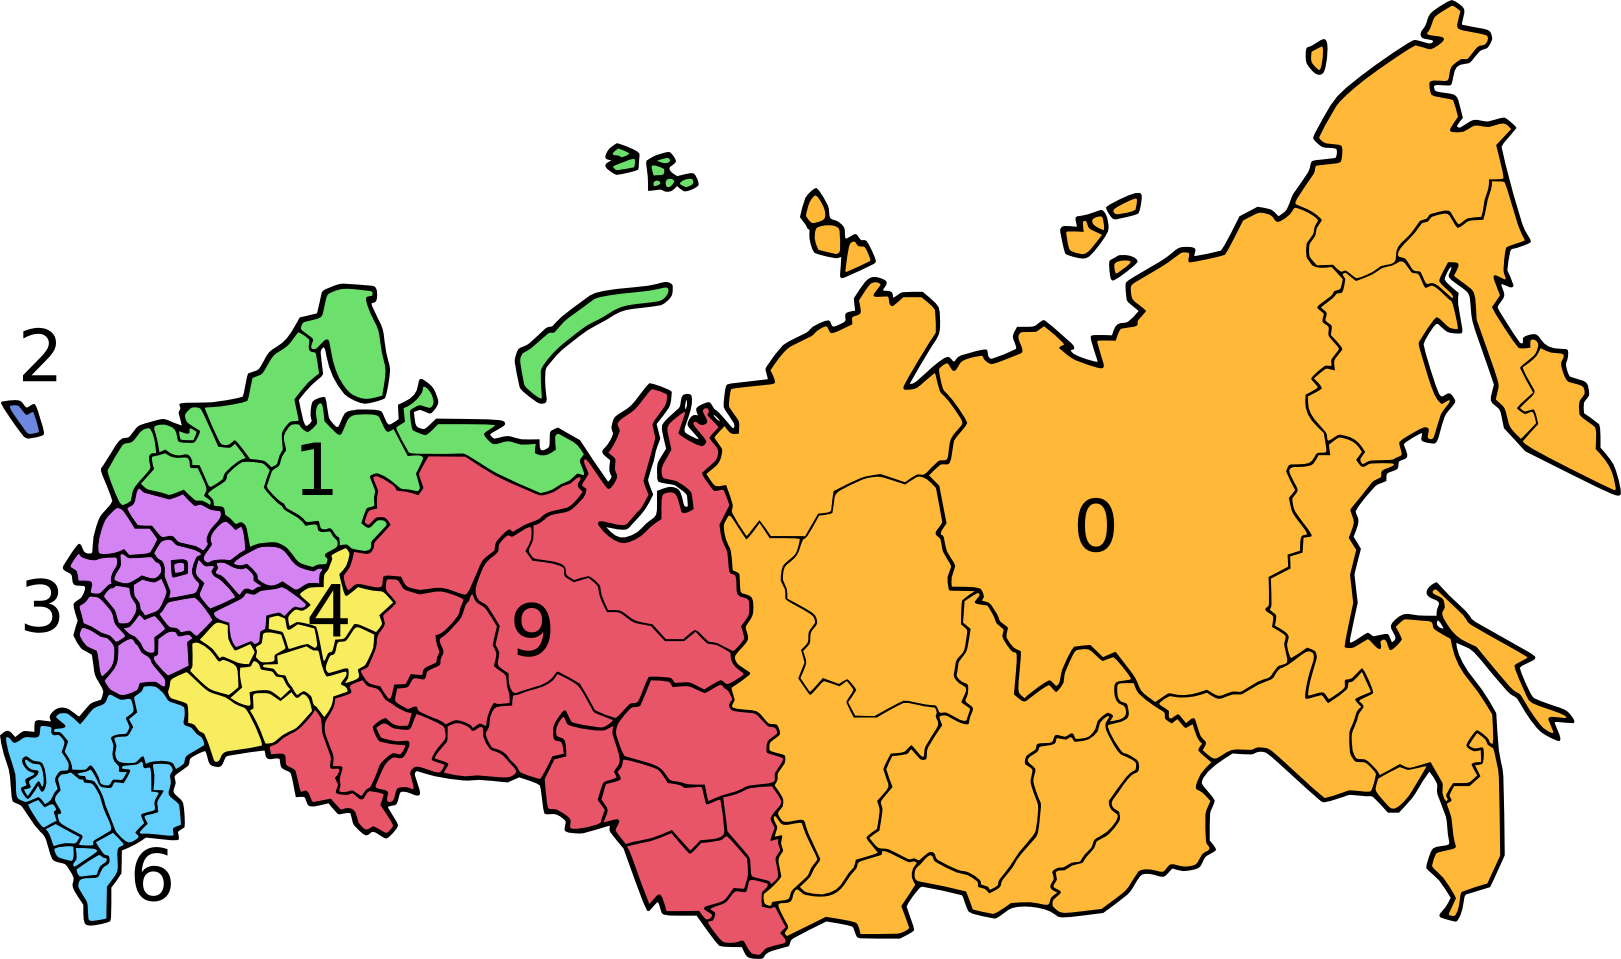
\includegraphics[width=8cm]{./png/Russia-amateur-callsign-districts.png}
 % Russia-amateur-callsign-districts.png: 1621x959 pixel, 90dpi, 45.77x27.08 cm, bb=0 0 1297 767
 \caption{Grobe Einteilung der Amateurfunk-Rufzeichen in Russland. \imgsrc{\href{http://en.wikipedia.org/wiki/File:Russia_amateur_callsign_districts.svg}{Chris Rovulo}, GFDL 1.2, cc-by-sa 3.0}}
 \label{fig:callsignsRU}
\end{figure}

\begin{figure}[h!]
 \centering
 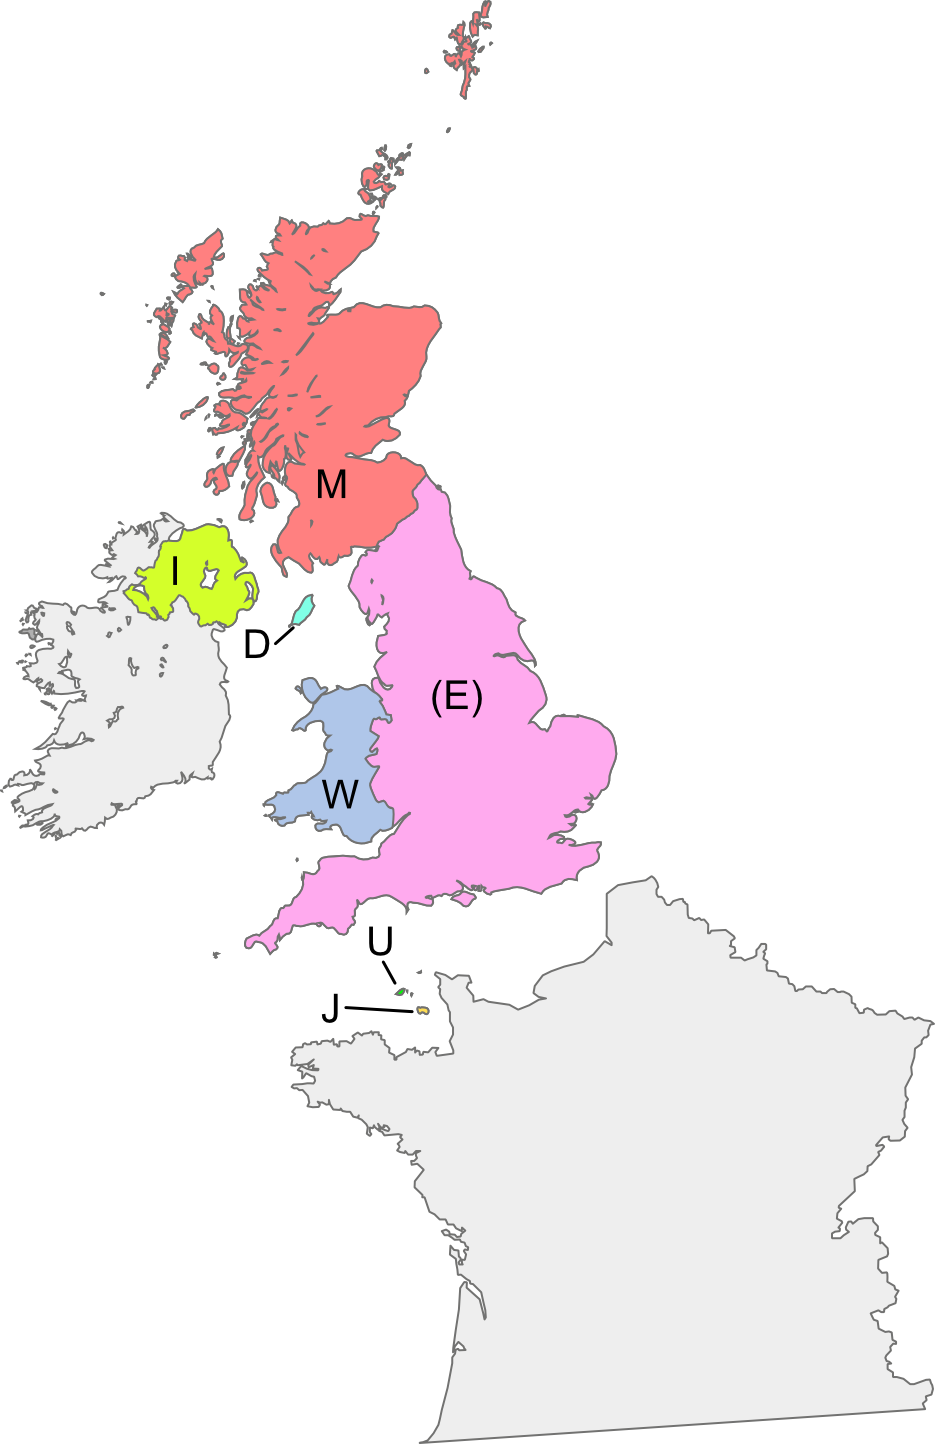
\includegraphics[height=6cm]{./png/UK-amateur-radio-regional-locators.png}
 % UK-amateur-radio-regional-locators.png: 935x1444 pixel, 90dpi, 26.39x40.76 cm, bb=0 0 748 1155
 \caption{Amateur-Rufzeichen in den UK. \imgsrc{\href{http://en.wikipedia.org/wiki/File:UK_amateur_radio_regional_locators.svg}{Adambro}, PD}}
 \label{fig:callsignsUK}
\end{figure}



\section{Kurzbeschrieb der Funkdienste}
\paragraph{Fixed Service} Dienst zwischen zwei festgelegten fixen Bodenstationen
\paragraph{Fixed — Satellite Service} Dienst zwischen Erdstation, wenn einer oder mehrere Satelliten benutzt werden
\paragraph{Mobile Service} Dienst zwischen mobilen und Landstationen oder zwischen mobilen Stationen
\paragraph{Mobile — Satellite Service} Dienst zwischen mobilen Erdstationen und einer oder mehreren Weltraumstationen oder zwischen Welt­raum­stationen
\paragraph{Maritime Mobile Service} Ein mobiler Dienst zwischen Küstenstationen und Schiffstationen oder zwischen Schiff­sta­tio­nen
\paragraph{Maritime Mobile — Satellite Service} Ein mobiler satellitengestützer Dienst, bei welchem sich mobile Erdstationen auf Schiffen befinden
\paragraph{Port-Operations Service} Ein mobiler Seefunk-Dienst in einem oder in der Nähe eines Hafens, zwischen Küstenstationen und Schiffstationen oder zwischen Schiffstationen
\paragraph{Aeronautical Mobile Service} Ein mobiler Dienst zwischen Flugbodenstationen und Luftfahrzeugen oder zwischen Luftfahr­zeugen
\paragraph{Broadcasting Service} Ein Dienst, bei welchem die Aussendungen für den direkten Empfang bei der Bevölkerung vorgesehen sind
\paragraph{Radio Amateur Service} Amateurfunk, wird von privaten Personen als Hobby betrieben







}

\chapter{Glossar}

\newcommand{\term}[2]{
\vspace{1em}\noindent {\large \bfseries \textsf{#1}} \vspace{.5em}\\
#2}


\term{AF}
{Audio Frequency, Töne im hörbaren Bereich. Auch NF (Niederfrequenz) genannt. 

Im Amateurfunk werden oftmals nur Frequenzen von 300 bis 3000 Hz übertragen, da dies für die Verständigung ausreichend ist und nicht übermässig viel Platz im Spektrum verschwendet. Die Bandbreite beträgt für ein solches Sprachsignal auf SSB $3000~\mathrm{Hz} - 300~\mathrm{Hz} = 2700~\mathrm{Hz}$.
}

\term{AGC}
{Der \textit{Automatic Gain Control} hält die AF auf einer bestimmten Stärke. Dies kann bei digitalen Übertragungsverfahren (RTTY, PSK) nützlich sein, da die Lautstärke konstant bleibt, bei CW ist er jedoch eher hinderlich, da während einer Sendepause das Rauschen gleich stark ist wie sonst das Signal.}

\term{AM}
{\link{Amplitudenmodulation, S. 35}}

\term{APRS}
{Automatic Position and Recording System – ein Zusammenspiel von GPS und Packet Radio.

144.800 MHz}

\term{Bake}
{Baken (wie zum Beispiel die \link{NCDXF-Baken, S. 26}) senden immer auf einer bestimmten Frequenz. So kann man sich ein Bild der aktuellen Ausbreitungsbedingungen machen.

Software: BeaconSee}

\term{Balun}
{Übergang von symmetrisch auf asymmetrisch (balanced – unbalanced). Beispiel: Übergang eines Dipols (symmetrisch) auf ein Koaxialkabel (asymmetrisch).}

\term{Beam}
{Siehe \link{Yagi}}

\term{Betriebsart}
{Die Betriebsart (also die Art, wie man Funkbetrieb macht) beinhaltet verschiedene Eigenschaften wie Verkehrsart (Simplex, Duplex, …), Modulation (AM, FM, …) und Übertragungsverfahren.}

\term{BFO}
{Der \textit{Beat Frequency Oscillator} generiert eine Trägerfrequenz, die bei Bedarf der ZF beigemischt wird. Beispielsweise wird dies bei CW oder SSB benötigt.

Im folgenden Beispiel wird ein CW-Signal dargestellt. 

%\begin{minipage}{55mm}
\begin{figure}[h!]
 \centering
 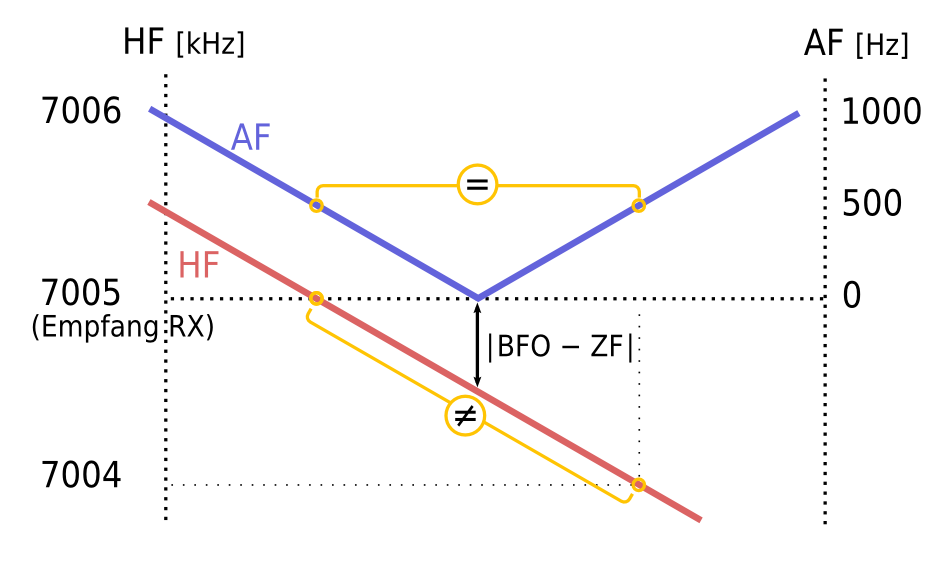
\includegraphics[width=5cm]{./png/Amfu-BFO.png}
 % Amfu-BFO.png: 929x581 pixel, 295dpi, 8.00x5.00 cm, bb=0 0 227 142
 \caption{Grosse Bandbreite: Ein CW-Signal auf 7005 kHz hat die selbe NF-Tonhöhe wie ein Signal auf 7004 kHz.}
 \label{fig:bfo}
\end{figure}
%\end{minipage}
%\begin{minipage}{55mm}
\begin{figure}[h!]
 \centering
 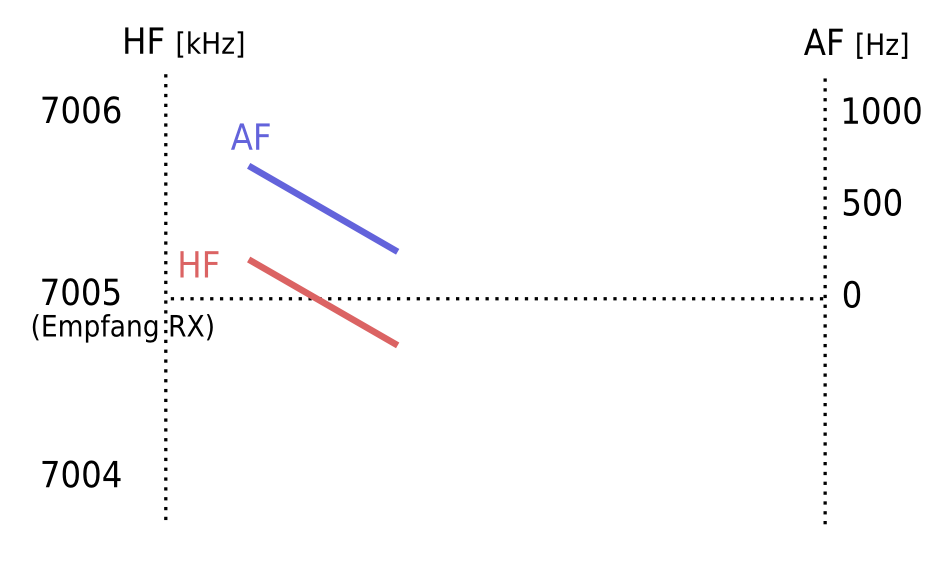
\includegraphics[width=5cm]{./png/Amfu-BFO-Filter.png}
 % Amfu-BFO-Filter.png: 929x581 pixel, 295dpi, 8.00x5.00 cm, bb=0 0 227 142
 \caption{Bei einer Bandbreite von 0.5 kHz verschwindet dieses Problem.}
 \label{fig:bfoFilter}
\end{figure}
%\end{minipage}



$f_d = |f_{\mathrm{BFO}}-f_{\mathrm{ZF}}|$ lässt sich beim Empfänger meist direkt einstellen. Ein Signal, das direkt auf der Empfangsfrequenz liegt, wird dann mit dieser NF hörbar gemacht. Andernfalls wird der Abstand zur Eingangsfrequenz addiert oder subtrahiert: $|f_d + (f_\mathrm{Signal}-f_\mathrm{RX})|$.

Das ist auch der Grund, warum beim Scannen eines CW-Bandes die einen Signale höher, die andern tiefer werden. Beim Empfang eines breiten Spektrums haben zwei Signale, die $2\times \mathrm{f_d}$ auseinander liegen, die selbe AF-Tonhöhe! Darum verschwinden einige Signale beim verringern der Bandbreite, da sie zwar die eingestellte fd-Tonhöhe haben, aber um die zweifache fd-Frequenz weiter unten liegen. Sobald die Bandbreite unter $2\times \mathrm{f_d}$  liegt, hat man diese Probleme nicht mehr.}

\term{Bodenwelle}
{\link{Bodenwelle, Seite 33}}

\term{CB}
{Abkürzung für \textit{Citizen Band}. Auf diesem HF-Band um 27 MHz kann, ähnlich wie bei PMR, ohne Lizenz gefunkt werden.}

\term{CTCSS}
{CTCSS \textit{(Continious Tone Code Squelch System)} moduliert einen NF-Ton unter 300 Hz (\link{Subaudio}-Ton) mit dem FM-Träger. CTCSS wird gerne von Relais benutzt, da damit ungewollte Aktivierungen, z. B. von Radars oder durch Nebenaussendungen anderer Stationen, verhindert werden können: Es öffnet nur, wenn der richtige Ton moduliert wird.

Insgesamt werden 50 verschiedene Töne von 67 bis 254.1 Hz verwendet.}

\term{Dämpfung}
{Die Dämpfung bzw. Verstärkung (Kabel, Antenne, …) wird in Dezibel (dB) angegeben. Für Koaxialkabel gilt der Wert jeweils für 100 m.}

\term{DCS}
{DCS (Digital Code Squelch) funktioniert ähnlich wie \link{CTCSS}: Der Empfänger wird geöffnet, sobald das richtige Signal am HF-Eingang liegt. DCS arbeitet jedoch mit einem FSK-Stream im Subaudio-Bereich, mit dem Daten (bzw. bestimmte Codes) übertragen werden. Das System ist so weniger störanfällig.}

\term{Dezibel}
{Es können sowohl relative Angaben zur Verstärkung bzw. Dämpfung als auch absolute bei Pegeln verwendet werden. dB-Werte sind addierbar, was die Errechnung des Gesamtgewinnes aus Antenne, Kabel- und Steckerverlust vereinfacht.
Bei der Angabe von Leistungspegeln gilt:

\[ a_\mathrm{dBm} = 10 \cdot \log \frac{P}{P_\mathrm{ref}} \]

Für Spannungspegel:

\[ a_\mathrm{dBµV} = 20 \cdot \log \frac{U}{U_\mathrm{ref}} \]

Eine Verstärkung der Leistung um 3 dB bedeutet eine Leistungsverdoppelung. Zwei Antennen mit je 3 dB Gewinn erbringen zusammen einen Gewinn von $3 + 3 = 6~\mathrm{dB}$ (also das Vierfache).

Nähere Beschreibung in der \link{Formelsammlung}.}

\term{DTMF}
{DTMF (Dual Tone Multiple Frequency), auch MFV – Mehrfrequenzwahlverfahren – genannt, wird zum aktivieren von Relais und für die Auswahl von \link{Echolink}-Repeatern verwendet. Die meisten EL-Relais verlangen zuerst einen \textbf{*}, um EL zu aktivieren, bevor die Node-Nummer eingegeben wird. Die Raute (\textbf{\#}) beendet die Verbindung wieder.}

\term{Dipol}
{Ein Antennendraht der Länge $\lambda/2$. Siehe \link{Dipol, Seite 42}.}

\term{Doppelsuper}
{Empfänger mit zwei Zwischenfrequenzen: Eine hohe erste ZF, die die Spiegelfrequenz unterdrückt, und eine zweite tiefe ZF, die eine gute Trennschärfe erlaubt. }

\term{Echolink}
{\href{http://www.echolink.org}{www.echolink.org} – Webauftritt von Echolink

Mit Echolink lassen sich Funkverbindungen zwischen zwei Benutzern «übers Internet» erstellen. Auf das Echolink-System kann man entweder vom PC aus\footnote{Software ist momentan nur für Windows erhältlich.} (VoIP-ähnlich) oder über ein Relais, das Echolink (EL) unterstützt, zugreifen. 

Sowohl Benutzer am PC als auch Relais bekommen eine ID zugewiesen. Zwischen zwei IDs kann eine Verbindung hergestellt werden; PC-Benutzer können so direkt angesprochen werden, auch über Funk.

Ein häufiger Verwendungszweck von Echolink ist die Erstellung einer Verbindung zwischen zwei Relais, die beliebig weit voneinander entfernt sein können, da Verbindungen zwischen zwei IDs digital übers Internet erfolgt.

\vspace{1em}
\begin{tabular}{ll}
\bfseries Input & \\ \toprule \arrayrulecolor{rowsep}
Nummer & Verbindet mit dem gewählten Node \\ \midrule
\# & Unterbricht die aktive Verbindung \\ \midrule
* & Stationsinfo, wenn nicht verbunden \\ \midrule
0 & Verbindet mit zufälliger Station jeden Typs \\ \midrule
1 & Verbindet mit zufälligem -L (Link) oder -R (Repeater) \\ \midrule
2 & Verbindet mit zufälligem Konferenzserver \\ \midrule
3 & Verbindet mit zufälligem Benutzer \\ \midrule
06 Nr. & Statusinfo zur gewählten Nummer \\ \midrule
8 & Gibt die Rufzeichen der verbundenen Stationen aus  \\ \midrule
9 & Wiederwahl zu zuletzt gewählter Station \\ \midrule
\end{tabular}
}


\term{FM}
{\link{Frequenzmodulation, S. 37}}

\term{FRS}
{Family Radio Service; Amerikanisches PMR.}

\term{Fuchsjagd}
{Amateurfunkpeilen. Ähnlich wie bei einem OL müssen Sender, die auf einer bestimmten Frequenz senden, gefunden werden. Durch mehrere Peilungen können sie geortet und auf einer Karte eingetragen werden. \link{Formelsammlung}}

\term{Ground wave}
{\link{Bodenwelle, Seite 33}}

\term{Hochpass}
{Filter aus Kondensatoren und Spulen, das hohe Frequenzen passieren lässt. Wird auch eingesetzt, um den 50-Hz-Brumm der Steckdose zu entfernen.}

\term{ITU}
{Die \textit{International Telecommunication Union}, auf Deutsch Internationale Fernmeldeunion. }

\term{Koax}
{Koaxialkabel wird für die Übertragung der Signale zwischen Antenne und Empfänger verwendet. Die gebräuchlichsten Arten sind RG58 (5.8 mm Durchmesser) und RG213 (10.3 mm Durchmesser).

Für Amateurfunk verwendet man eigentlich nur 50-$\Omega$-Kabel. 75-Ohmiges wird im Fernsehbereich eingesetzt.

Aufgrund des \link{Skin-Effektes} wird bei höheren Frequenzen dickeres Kabel (RG213) eingesetzt.
}

\term{Koax-Steckverbindungen}
{Häufige Steckverbindungen: BNC, N und UHF/PL. BNC findet man oft an RG58-Kabel, N wird eher für das dicke RG213 verwendet (VHF/UHF). PL-Stecker sind nur für Frequenzen bis ungefähr 200 MHz geeignet.}

\term{Kyrillisch}
{Im kyrillischen Alphabet haben «unsere» Buchstaben eine andere Bedeutung. In folgender Tabelle jeweils links der kyrillische Buchstabe und rechts das lateinische Morsezeichen (die Morsezeichen sind in den Bakom-Vorschriften angegeben).

\vspace{1em}
\begin{tabular}{l>{\bfseries}l l>{\bfseries}l l>{\bfseries}l}
\ru{А а} & a & \ru{К к} & k & \ru{Х х} & h \\ \midrule
\ru{Б б} & b & \ru{Л л} & l & \ru{Ц ц} & c \\ \midrule
\ru{В в} & w & \ru{М м} & m & \ru{Ч ч} & ö \\ \midrule
\ru{Г г} & g & \ru{Н н} & n & \ru{Ш ш} & ch \\ \midrule
\ru{Д д} & d & \ru{О о} & o & \ru{Щ щ} & q \\ \midrule
\ru{Е е} & e & \ru{П п} & p & \ru{Ъ ъ} & x \\ \midrule
\ru{Ё ё} & e & \ru{Р р} & r & \ru{Ы ы} & y \\ \midrule
\ru{Ж ж} & v & \ru{С с} & s & \ru{Ь ь} & x \\ \midrule
\ru{З з} & z & \ru{Т т} & t & \ru{Э э} & é \\ \midrule
\ru{И и} & i & \ru{У у} & u & \ru{Ю ю} & ü \\ \midrule
\ru{Й й} & j & \ru{Ф ф} & f & \ru{Я я} & ä \\ \midrule
\end{tabular}


}

\term{Locator}
{\link{Maidenhead-Locator}}

\term{LUF}
{Die Lowest Usable Frequency ist die tiefste Frequenz, die zwischen zwei Punkten genutzt werden kann. Sie ist von der Ionisierung der D- und E-Schicht und daher auch von der Tageszeit abhängig.}

\term{Maidenhead-Locator}
{Im Amateurfunk wird für die Positionsangabe ein eigenes System verwendet. Die Welt wird in $18\times 18$ Grösstfelder (\textit{Fields}, A…R), $10\times 10$ Grossfelder (\textit{Squares}, 0…9) und $24\times 24$ Kleinfelder (\textit{Subsquares}, a…x) unterteilt, feinere Unterteilungen sind möglich. Das erste Zeichen gibt jeweils die Länge an, das zweite die Breite. Beispiel: JN47qh

\begin{figure}[h!]
 \centering
 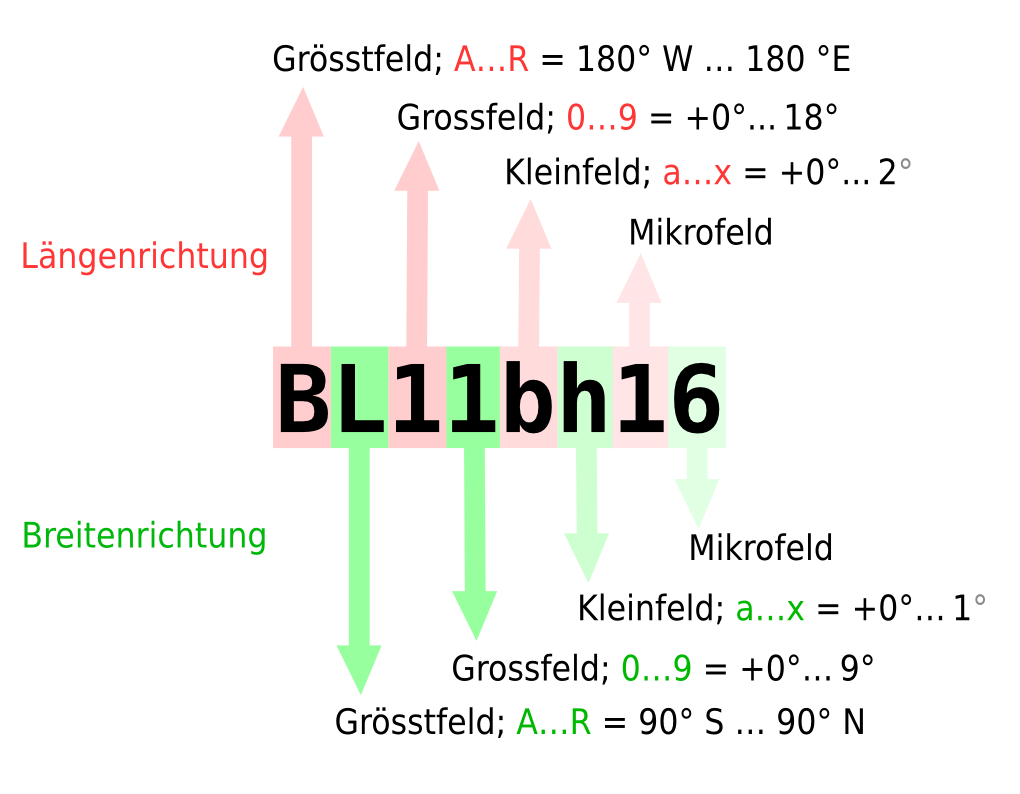
\includegraphics[width=6cm]{./png/Maidenhead_QTH-Locator_erklaert.png}
 \caption{Aufbau des Maidenhead-Locators}
 \label{fig:maidenhead}
\end{figure}

}

\term{Modulationsindex}
{Verhältnis von Hubfrequenz zur maximalen Niederfrequenz}

\term{MUF}
{Die Maximal Usable Frequency liegt wenig unter der höchsten Frequenz, die an der F-Schicht der Ionosphäre noch reflektiert wird. Tagsüber ist sie höher als bei Nacht. Ausserdem ist sie abhängig vom Abstrahlwinkel: Bei sehr guten Bedingungen und einem Abstrahlwinkel um 0° können Frequenzen von bis zu 70 MHz reflektiert werden.

Sonden, die die MUF messen, senden ein Signal zur Erde, das dann reflektiert wird. Da es senkrecht auf die Ionosphäre auftrifft, ist die so erhaltene MUF niedriger. Die 0°-MUF kann daraus hochgerechnet werden – für das $F_2$-Band beträgt sie das 2.5- bis 3.5-fache.}

\term{Netzeinströmung}
{Beim Senden kann es geschehen, dass ein Teil der Energie ins Stromnetz einströmt und so zu Störungen anderer Geräte führt. Dies kann verhindert werden, indem man das Stromkabel um einen Ferritring wickelt. Grundsätzlich gilt: Je mehr Windungen, desto besser, aber ein Viertel des Ferrites sollte frei bleiben.}

\term{NF}
{\link{AF}}

\term{Notchfilter}
{Ein Notchfilter (Saugkreis) filtert eine HF-Frequenz heraus.

\begin{figure}[h!]
 \centering
 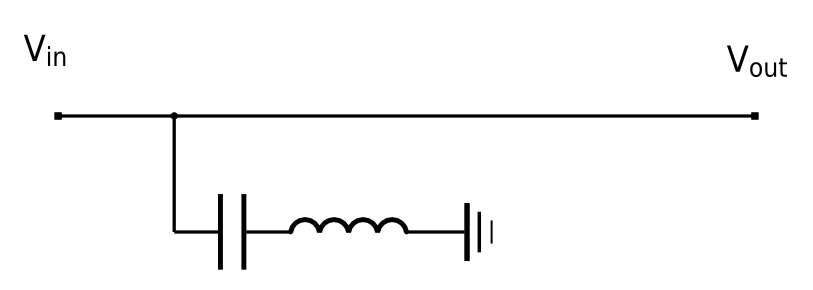
\includegraphics[width=4cm]{./png/Amfu-Schema-Notchfilter.png}
 % Amfu-Schema-Notchfilter.png: 813x290 pixel, 295dpi, 7.00x2.50 cm, bb=0 0 198 71
 \caption{Einfacher Notchfilter: Serieschwingkreis}
 \label{fig:notchfilter}
\end{figure}

Nach dem selben Prinzip funktionieren einstellbare, schmalbandigere Notchfilter später im Empfänger. Dies ist vor allem nützlich, wenn eine andere Station stört.

Ein einfacher Notchfilter lässt sich mit einer Spule und einem Kondensator realisieren, die in Serie geschaltet und zwischen Antenne und Erde gehängt werden. Für den NF-Bereich wird anstelle einer Spule ein Widerstand eingebaut, da für tiefe Frequenzen eine grosse Induktivität notwendig wäre.

\begin{figure}[h!]
 \centering
 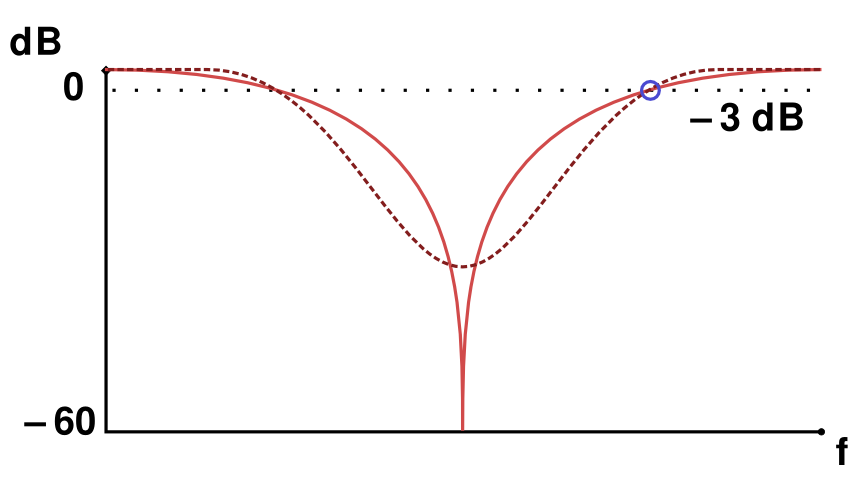
\includegraphics[width=5cm]{./png/Amfu-Notchfilter.png}
 % Amfu-Notchfilter.png: 864x480 pixel, 288dpi, 7.62x4.23 cm, bb=0 0 216 120
 \caption{Dämpfungskurven: Notchfilter und 
(gestrichelt) Bandsperre}
 \label{fig:notchfilterFreq}
\end{figure}
}

\term{Öffnungswinkel}
{Der Öffnungswinkel einer Antenne ist der Winkelabstand zwischen zwei Punkten, bei denen der Gewinn um 3 dB abgefallen ist. Ein Yagi hat einen kleineren Öffnungswinkel als ein Dipol.}

\term{Ortung}
{Positionsbestimmung eines Signals durch zwei oder mehr \link{Peilungen}.}

\term{Peilung}
{Richtungsbestimmung eines Signals. Für \link{Fuchsjagden} wird dazu meist eine Loop verwendet, für HF werden stationäre Peiler mit mehreren GPs, in einem Kreis angeordnet, eingesetzt.}

\term{Pile-up}
{Ein Effekt, der bei speziellen Stationen oder bei Contests auftritt, wenn mehrere Stationen mit einer bestimmten eine Verbindung herstellen möchten.}

\term{PMR}
{PMR \textit{(Private Mobile Radio)} bezeichnet den «Funk für Jedermann»: Hier darf ohne Amateurfunklizenz gefunkt werden. Auf den PMR-Geräten sind 8 verschiedene Kanäle verfügbar, auf denen mit FM und halbem Hub (für eine geringere Leistungsaufnahme und höhere Kanaldichte) gefunkt wird.

Auf den PMR-Frequenzen (446–446.1 MHz) dürfen alle geprüften PMR-Handfunkgeräte mit bis zu 500 mW senden. Amateurfunkgeräte sind normalerweise nicht für diese Kanäle geprüft und erlauben es darum im unmodifizierten Zustand auch nicht, dort zu funken.}

\term{Polarisation}
{Bei Antennen unterscheidet man zwischen horizontaler und vertikaler Polarisation des elektrischen Feldes. Für einen optimalen Empfang sollte die Polarisation zweier Stationen übereinstimmen. Dipole sind grundsätzlich horizontal, GPs vertikal polarisiert.

\begin{figure}[h!]
 \centering
 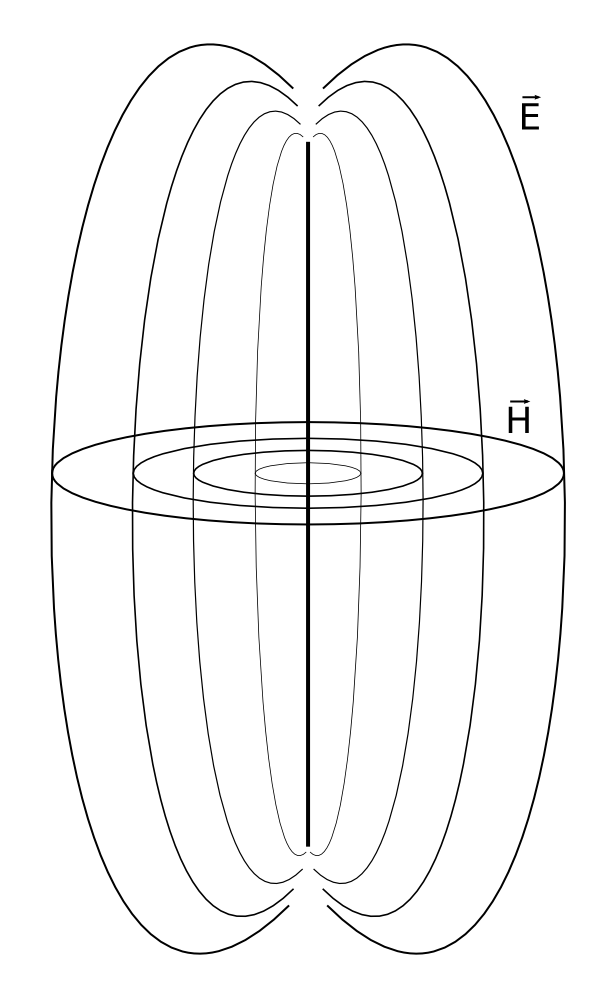
\includegraphics[height=5cm]{./png/Amfu-Antenne-Polarisation.png}
 % Amfu-Antenne-Polarisation.png: 612x1008 pixel, 360dpi, 4.32x7.11 cm, bb=0 0 122 202
 \caption{GP, vertikal polarisiert}
 \label{fig:polarisation}
\end{figure}

}

\term{QRN}
{QRN entsteht durch atmosphärische Störungen wie Gewitter (Blitze sind auf dem gesamten Spektrum hörbar!) und kann den Funkverkehr erheblich beeinträchtigen. Andererseits kann genau dies zum Beispiel auch zum Zählen von Blitzen verwendet werden.

Nicht zu verwechseln mit QRM \textit{(man-made noise)}, Störungen, die etwa durch ein schlechtes Netzteil (Brummton) oder diverse elektrische Geräte hervorgerufen werden können.}

\term{Raumwelle}
{\link{Raumwelle, Seite 33}}

\term{Rauschsperre}
{Squelch}

\term{RG-58}
{Koaxialkabeltyp, der gerne für HF eingesetzt wird.}

\term{RIT}
{Das \textit{Receiver Incremental Tuning} (auch \textit{Clarifier} genannt) wird eingesetzt, wenn eine empfangene Station keinen stabilen Sender hat und sich dessen Frequenz langsam verändert (die von ihm empfangene Frequenz jedoch nicht!). Beim RIT wird nur die Eingangsfrequenz verstellt; so ist es möglich, auf der selben Frequenz zu senden, aber etwas daneben zu hören.

RIT wird oft auch von raren DX-peditions gebraucht, welche nach dem CQ-Ruf z. B. «up 2» geben (das heisst, sie wollen, dass man sie 2 kHz weiter oben ruft, um das Pile-up besser in
den Griff zu bekommen).}

\term{Schwund}
{Wird von einem Signal mehr als eine Reflexion empfangen, führt das zu starken Schwankungen der Signalstärke.}

\term{Sferics}
{Kommt von \textit{atmospherics}. \link{Blitze, Seite 34}}

\term{Signal-Rausch-Abstand}
{SNR. \link{Formelsammlung}}

\term{Skin-Effekt}
{Ein Leiter (zum Beispiel ein Kupferkabel) zeigt bei Gleichstrom eine gleichmässige Stromverteilung. Bei Wechselstrom werden die Elektronen aufgrund des Magnetfeldes, das durch die Mitte des Leiters geht, nach aussen verdrängt. So steigt der Widerstand etwa bei 10 MHz bereits um das 10-fache an (Kupferdraht, $1~\mathrm{mm}^2$). Abhilfe schafft Litzendraht (mehrere feine Drähte haben leicht bessere Eigenschhaften) oder, noch besser, ein dickerer Leiter.}

\term{Sky wave}
{\link{Raumwelle, Seite 33}}

\term{Spektrogramm}
{Ein Spektrogramm, beziehungsweise eine Spektrumanalyse, zeigt zu einer bestimmten Zeitspanne die Verteilung der Signalstärken im analysierten Frequenzband auf. Beispiel: \link{Grafik 5, Seite 36.}

Berechnet wird das Spektrogramm mittels FFT \textit{(Fast Fourier Transformation)}. Frequenz und Zeit können dabei aufgrund der Unschärferelation nicht gleichzeitig exakt bestimmt werden.}

\term{Sperrkreis}
{Der Sperrkreis (Parallelschwingkreis) hat eine andere Dämpfungskurve als der \link{Notchfilter}. Sie werden oft zusammen verwendet.

\begin{figure}[h!]
 \centering
 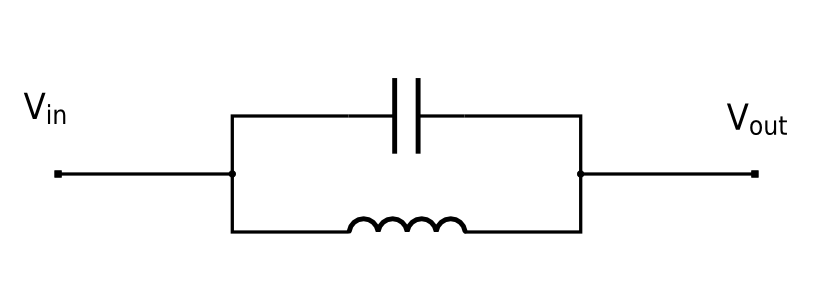
\includegraphics[width=4cm]{./png/Amfu-Schema_Sperrkreis.png}
 % Amfu-Schema_Sperrkreis.png: 813x290 pixel, 295dpi, 7.00x2.50 cm, bb=0 0 198 71
 \caption{Schaltschema einer Bandsperre}
 \label{fig:sperrkreis}
\end{figure}

}

\term{Squelch}
{Der Squelch (Rauschsperre) sperrt den NF-Verstärker, solange das Signal im ZF-Verstärker einen bestimmten, einstellbaren Wert nicht überschreitet. So ist der Empfang etwas angenehmer (speziell für FM), da bei Sendepausen kein Rauschen hörbar ist, und bei Handfunkgeräten wird die Betriebsdauer verlängert. Bei schwachen Signalen, die unter dem Rauschpegel liegen, funktioniert der Squelch nicht (bzw. sperrt immer).

Bei oft benutzten Relais kann man zudem mit einem \link{Subaudio-Ton} arbeiten, der am Gerät eingestellt wird. Der Empfänger verstärkt dann nur empfangene Aussendungen, die diesen CTCSS-Ton enthalten \textit{(Tone Squelch)}. Die Frequenzen dieser «privaten» CTCSS-Töne werden untereinander ausgetauscht.

Die Rauschsperre findet vor allem bei FM Einsatz, da das Rauschen lauter als das Sprachsignal ist. Bei AM wird sie zum Sperren von Störungen verwendet.}

\term{SSB}
{\link{SSB, S. 37}}

\term{Subaudio-Ton}
{Ein Ton, dessen Frequenz unterhalb der hörbaren Frequenzen (\link{AF}) liegt. Er kann etwa zur Datenübertragung mitgesendet werden.}

\term{SWR}
{Stehwellenverhältnis, auch VSWR für Vorwärts-SWR. Je höher das SWR, desto mehr Leistung wird von der Antenne zurückgeworfen und geht als Wärme verloren. Es wird berechnet, indem man die maximale durch die minimale Leistung teilt:

\[\mathrm{SWR} = \frac{U_\mathrm{hin} + U_\mathrm{rück}}{U_\mathrm{hin}-U_\mathrm{rück}}\]
}

\term{Tiefpass}
{Wie ein Hochpass, lässt aber tiefe Frequenzen passieren. \link{Formelsammlung}}

\term{Tone Call}
{Auch \textit{T-Call} genannt. Ein Ton mit einer Frequenz von 1750 Hz, der zum Aktivieren von Relais verwendet werden kann.}

\term{Tote Zone}
{Die tote Zone ist ein Bereich zwischen dem Ende der Bodenwelle und dem ersten Auftreffen der reflektierten Raumwelle, in dem ein Signal nicht empfangen werden kann.}

\term{Tuner}
{Ein Gerät, das die Ausgangsimpedanz des Senders an die Impedanz der Antenne anpasst, um so eine optimale Leistungsübertragung zu ermöglichen.}

\term{Übertragungsverfahren}
{Bezeichnet die Art, wie etwas übertragen wird. Als Beispiel: CW, SSTV, PSK31. \link{Übertragungsverfahren, Seite 40} und \link{Betriebsart}}

\term{UTC}
{\link{UTC, Seite 10}}

\term{Verkürzungsfaktor}
{Elektromagnetische Signale bewegen sich nur im luftleeren Raum mit Lichtgeschwindigkeit fort. In anderen Materialien (speziell Antennendraht und -Kabel) ist die Fortbewegungsgeschwindigkeit niedriger, daher muss zum Beispiel die Drahtlänge eines 80-m-Dipols um einen Meter verkürzt werden.}

\term{Verstärkung}
{\link{Dämpfung}}

\term{Wasserfalldiagramm}
{Der Wasserfall ist eine erweiterte Form des Spektrogramms. Die Signalstärke wird farblich hervorgehoben, dafür wird die dadurch frei gewordene Achse als Zeitachse verwendet. So ist es möglich, Frequenz, Zeit und Signalstärke gleichzeitig in einer zweidimensionalen Grafik darzustellen.  Beispiel: \link{Grafik 12, Seite 40}. \link{Spektrogramm}.

Heute findet der Wasserfall speziell bei digitalen Übertragungsverfahren wie PSK31 Verwendung, da so einzelne PSK-Signale schnell erkannt werden können.}

\term{Yagi}
{Eine \link{Yagi (S. 43)} ist eine Richtantenne.}

\term{Zwischenfrequenz}
{Die Zwischenfrequenz (ZF) ist der Abstand von der Oszillator- zur Eingangsfrequenz bzw. von der Oszillator- zur Spiegel­fre­quenz.}

\chapter{Internetseiten}

\paragraph{ham.granjow.net} Die Seite zu diesem Behelf.

\paragraph{USKA} Union Schweizerischer Kurzwellen-Amateure. Anlaufstelle für zukünfige Amateurfunker. \href{http://www.uska.ch}{www.uska.ch}

\paragraph{IARU} International Amateur Radio Union. \href{http://www.iaru.org}{www.iaru.org}

\paragraph{Wikipedia} \href{http://de.wikipedia.org}{http://de.wikipedia.org}

\paragraph{Bakom} \href{http://www.bakom.ch}{www.bakom.ch}

\paragraph{CEPT} \href{http://www.cept.org}{www.cept.org}

\paragraph{Weaksignals} Diverse Programme wie Spectran für den Amateurfunk. \href{http://www.weaksignals.com}{www.weaksignals.com}

\paragraph{PSKmail} \href{http://pskmail.wikispaces.com}{http://pskmail.wikispaces.com}

\chapter{Programme}

\section{Linux}
\paragraph{Baudline} Sehr umfangreiche Spektrumanalyse mit vielen Anzeigen (wie Spektrum, Wasserfall, Durchschnitt) und Einstellungsmöglichkeiten wie ein Rauschfilter. Beispiel: \link{Grafik 12, RTTY-Wasserfall}.

\paragraph{extcalc} Rechner, der auch zur grafischen Darstellung von Modulationen verwendet werden kann. Unterstützt Integral etc. Beispiel: \link{Grafik 4 zur Amplitudenmodulation}.

\paragraph{FFTExplorer} Spektrumanalyse mit der Möglichkeit, gewisse Signale zu generieren und zu modulieren (AM/FM). \href{http://www.arachnoid.com}{www.arachnoid.com}

Auf der Seite sind ausserdem weitere interessante Programme zu finden wie eines zum lokalisieren von Satelliten oder zum generieren von Tönen.

\paragraph{japa} (JACK and ALSA Perceptual Analyser) Spektrumanalyse (z.\,B. \link{Grafik 5}, AM-Signal mit dem typischen Peak des Trägersignals). \href{http://www.kokkinizita.net/linuxaudio/}{www.kokkinizita.net/linuxaudio/}

\paragraph{jaaa} (JACK and ALSA Audio Analyser) Ähnlich wie japa, selber Link.

\paragraph{Audacity} Audio-Editor. Auch für Mac und Windows verfügbar. Beispiel: \link{Grafik 13}, Ausschnitt eines PSK31-Datenstroms. \href{http://www.audacity.de}{www.audacity.de}

\section{Windows}
\paragraph{SpecLab 20001} Wasserfall- und andere Diagramme, Analysemöglichkeiten

\paragraph{4nec212} Antennensimulationsprogramm. \href{http://home.ict.nl/$\sim$arivoors/}{http://home.ict.nl/$\sim$arivoors/}

\paragraph{Great Circular Maps12} Projiziert ein Maidenhead-Locator-Netz auf die Erdkugel. \href{http://hem.passagen.se/sm3gsj/gcm/download.htm}{http://hem.passagen.se/sm3gsj/gcm/download.htm}

\chapter{Bildnachweis}
\noindent
\textsc{Anja Ballschmieter} [Deutschland]: Amateurfunk-Logo auf der Titelseite\\
\textsc{Oona} [Finnland]: Grafik 21\\
\textsc{Simon A. Eugster}: Restliche Grafiken. Die Zeichnungen wurden mit dem freien Vektorgrafikprogramm Inkscape erstellt. \href{http://www.inkscape.org}{www.inkscape.org}

\chapter{Notizen}


\chapter*{\rlap{GNU Free Documentation License}}\label{sec:gfdl}
\phantomsection  % so hyperref creates bookmarks
\addcontentsline{toc}{chapter}{GNU Free Documentation License}

\tiny
\begin{multicols}{2}

 \begin{center}

       Version 1.3, 3 November 2008


 Copyright \copyright{} 2000, 2001, 2002, 2007, 2008  Free Software Foundation, Inc.
 
 \bigskip
 
     \texttt{<http://fsf.org/>}
  
 \bigskip
 
 Everyone is permitted to copy and distribute verbatim copies
 of this license document, but changing it is not allowed.
\end{center}


\begin{center}
{\bf\footnotesize Preamble}
\end{center}

The purpose of this License is to make a manual, textbook, or other
functional and useful document ``free'' in the sense of freedom: to
assure everyone the effective freedom to copy and redistribute it,
with or without modifying it, either commercially or noncommercially.
Secondarily, this License preserves for the author and publisher a way
to get credit for their work, while not being considered responsible
for modifications made by others.

This License is a kind of ``copyleft'', which means that derivative
works of the document must themselves be free in the same sense.  It
complements the GNU General Public License, which is a copyleft
license designed for free software.

We have designed this License in order to use it for manuals for free
software, because free software needs free documentation: a free
program should come with manuals providing the same freedoms that the
software does.  But this License is not limited to software manuals;
it can be used for any textual work, regardless of subject matter or
whether it is published as a printed book.  We recommend this License
principally for works whose purpose is instruction or reference.


\begin{center}
{\small\bf 1. APPLICABILITY AND DEFINITIONS\par}
\phantomsection
\end{center}

This License applies to any manual or other work, in any medium, that
contains a notice placed by the copyright holder saying it can be
distributed under the terms of this License.  Such a notice grants a
world-wide, royalty-free license, unlimited in duration, to use that
work under the conditions stated herein.  The ``\textbf{Document}'', below,
refers to any such manual or work.  Any member of the public is a
licensee, and is addressed as ``\textbf{you}''.  You accept the license if you
copy, modify or distribute the work in a way requiring permission
under copyright law.

A ``\textbf{Modified Version}'' of the Document means any work containing the
Document or a portion of it, either copied verbatim, or with
modifications and/or translated into another language.

A ``\textbf{Secondary Section}'' is a named appendix or a front-matter section of
the Document that deals exclusively with the relationship of the
publishers or authors of the Document to the Document's overall subject
(or to related matters) and contains nothing that could fall directly
within that overall subject.  (Thus, if the Document is in part a
textbook of mathematics, a Secondary Section may not explain any
mathematics.)  The relationship could be a matter of historical
connection with the subject or with related matters, or of legal,
commercial, philosophical, ethical or political position regarding
them.

The ``\textbf{Invariant Sections}'' are certain Secondary Sections whose titles
are designated, as being those of Invariant Sections, in the notice
that says that the Document is released under this License.  If a
section does not fit the above definition of Secondary then it is not
allowed to be designated as Invariant.  The Document may contain zero
Invariant Sections.  If the Document does not identify any Invariant
Sections then there are none.

The ``\textbf{Cover Texts}'' are certain short passages of text that are listed,
as Front-Cover Texts or Back-Cover Texts, in the notice that says that
the Document is released under this License.  A Front-Cover Text may
be at most 5 words, and a Back-Cover Text may be at most 25 words.

A ``\textbf{Transparent}'' copy of the Document means a machine-readable copy,
represented in a format whose specification is available to the
general public, that is suitable for revising the document
straightforwardly with generic text editors or (for images composed of
pixels) generic paint programs or (for drawings) some widely available
drawing editor, and that is suitable for input to text formatters or
for automatic translation to a variety of formats suitable for input
to text formatters.  A copy made in an otherwise Transparent file
format whose markup, or absence of markup, has been arranged to thwart
or discourage subsequent modification by readers is not Transparent.
An image format is not Transparent if used for any substantial amount
of text.  A copy that is not ``Transparent'' is called ``\textbf{Opaque}''.

Examples of suitable formats for Transparent copies include plain
ASCII without markup, Texinfo input format, LaTeX input format, SGML
or XML using a publicly available DTD, and standard-conforming simple
HTML, PostScript or PDF designed for human modification.  Examples of
transparent image formats include PNG, XCF and JPG.  Opaque formats
include proprietary formats that can be read and edited only by
proprietary word processors, SGML or XML for which the DTD and/or
processing tools are not generally available, and the
machine-generated HTML, PostScript or PDF produced by some word
processors for output purposes only.

The ``\textbf{Title Page}'' means, for a printed book, the title page itself,
plus such following pages as are needed to hold, legibly, the material
this License requires to appear in the title page.  For works in
formats which do not have any title page as such, ``Title Page'' means
the text near the most prominent appearance of the work's title,
preceding the beginning of the body of the text.

The ``\textbf{publisher}'' means any person or entity that distributes
copies of the Document to the public.

A section ``\textbf{Entitled XYZ}'' means a named subunit of the Document whose
title either is precisely XYZ or contains XYZ in parentheses following
text that translates XYZ in another language.  (Here XYZ stands for a
specific section name mentioned below, such as ``\textbf{Acknowledgements}'',
``\textbf{Dedications}'', ``\textbf{Endorsements}'', or ``\textbf{History}''.)  
To ``\textbf{Preserve the Title}''
of such a section when you modify the Document means that it remains a
section ``Entitled XYZ'' according to this definition.

The Document may include Warranty Disclaimers next to the notice which
states that this License applies to the Document.  These Warranty
Disclaimers are considered to be included by reference in this
License, but only as regards disclaiming warranties: any other
implication that these Warranty Disclaimers may have is void and has
no effect on the meaning of this License.


\begin{center}
{\small\bf 2. VERBATIM COPYING\par}
\phantomsection
\end{center}

You may copy and distribute the Document in any medium, either
commercially or noncommercially, provided that this License, the
copyright notices, and the license notice saying this License applies
to the Document are reproduced in all copies, and that you add no other
conditions whatsoever to those of this License.  You may not use
technical measures to obstruct or control the reading or further
copying of the copies you make or distribute.  However, you may accept
compensation in exchange for copies.  If you distribute a large enough
number of copies you must also follow the conditions in section~3.

You may also lend copies, under the same conditions stated above, and
you may publicly display copies.


\begin{center}
{\small\bf 3. COPYING IN QUANTITY\par}
\phantomsection
\end{center}


If you publish printed copies (or copies in media that commonly have
printed covers) of the Document, numbering more than 100, and the
Document's license notice requires Cover Texts, you must enclose the
copies in covers that carry, clearly and legibly, all these Cover
Texts: Front-Cover Texts on the front cover, and Back-Cover Texts on
the back cover.  Both covers must also clearly and legibly identify
you as the publisher of these copies.  The front cover must present
the full title with all words of the title equally prominent and
visible.  You may add other material on the covers in addition.
Copying with changes limited to the covers, as long as they preserve
the title of the Document and satisfy these conditions, can be treated
as verbatim copying in other respects.

If the required texts for either cover are too voluminous to fit
legibly, you should put the first ones listed (as many as fit
reasonably) on the actual cover, and continue the rest onto adjacent
pages.

If you publish or distribute Opaque copies of the Document numbering
more than 100, you must either include a machine-readable Transparent
copy along with each Opaque copy, or state in or with each Opaque copy
a computer-network location from which the general network-using
public has access to download using public-standard network protocols
a complete Transparent copy of the Document, free of added material.
If you use the latter option, you must take reasonably prudent steps,
when you begin distribution of Opaque copies in quantity, to ensure
that this Transparent copy will remain thus accessible at the stated
location until at least one year after the last time you distribute an
Opaque copy (directly or through your agents or retailers) of that
edition to the public.

It is requested, but not required, that you contact the authors of the
Document well before redistributing any large number of copies, to give
them a chance to provide you with an updated version of the Document.


\begin{center}
{\small\bf 4. MODIFICATIONS\par}
\phantomsection
\end{center}

You may copy and distribute a Modified Version of the Document under
the conditions of sections 2 and 3 above, provided that you release
the Modified Version under precisely this License, with the Modified
Version filling the role of the Document, thus licensing distribution
and modification of the Modified Version to whoever possesses a copy
of it.  In addition, you must do these things in the Modified Version:

\begin{itemize}
\item[A.] 
   Use in the Title Page (and on the covers, if any) a title distinct
   from that of the Document, and from those of previous versions
   (which should, if there were any, be listed in the History section
   of the Document).  You may use the same title as a previous version
   if the original publisher of that version gives permission.
   
\item[B.]
   List on the Title Page, as authors, one or more persons or entities
   responsible for authorship of the modifications in the Modified
   Version, together with at least five of the principal authors of the
   Document (all of its principal authors, if it has fewer than five),
   unless they release you from this requirement.
   
\item[C.]
   State on the Title page the name of the publisher of the
   Modified Version, as the publisher.
   
\item[D.]
   Preserve all the copyright notices of the Document.
   
\item[E.]
   Add an appropriate copyright notice for your modifications
   adjacent to the other copyright notices.
   
\item[F.]
   Include, immediately after the copyright notices, a license notice
   giving the public permission to use the Modified Version under the
   terms of this License, in the form shown in the Addendum below.
   
\item[G.]
   Preserve in that license notice the full lists of Invariant Sections
   and required Cover Texts given in the Document's license notice.
   
\item[H.]
   Include an unaltered copy of this License.
   
\item[I.]
   Preserve the section Entitled ``History'', Preserve its Title, and add
   to it an item stating at least the title, year, new authors, and
   publisher of the Modified Version as given on the Title Page.  If
   there is no section Entitled ``History'' in the Document, create one
   stating the title, year, authors, and publisher of the Document as
   given on its Title Page, then add an item describing the Modified
   Version as stated in the previous sentence.
   
\item[J.]
   Preserve the network location, if any, given in the Document for
   public access to a Transparent copy of the Document, and likewise
   the network locations given in the Document for previous versions
   it was based on.  These may be placed in the ``History'' section.
   You may omit a network location for a work that was published at
   least four years before the Document itself, or if the original
   publisher of the version it refers to gives permission.
   
\item[K.]
   For any section Entitled ``Acknowledgements'' or ``Dedications'',
   Preserve the Title of the section, and preserve in the section all
   the substance and tone of each of the contributor acknowledgements
   and/or dedications given therein.
   
\item[L.]
   Preserve all the Invariant Sections of the Document,
   unaltered in their text and in their titles.  Section numbers
   or the equivalent are not considered part of the section titles.
   
\item[M.]
   Delete any section Entitled ``Endorsements''.  Such a section
   may not be included in the Modified Version.
   
\item[N.]
   Do not retitle any existing section to be Entitled ``Endorsements''
   or to conflict in title with any Invariant Section.
   
\item[O.]
   Preserve any Warranty Disclaimers.
\end{itemize}

If the Modified Version includes new front-matter sections or
appendices that qualify as Secondary Sections and contain no material
copied from the Document, you may at your option designate some or all
of these sections as invariant.  To do this, add their titles to the
list of Invariant Sections in the Modified Version's license notice.
These titles must be distinct from any other section titles.

You may add a section Entitled ``Endorsements'', provided it contains
nothing but endorsements of your Modified Version by various
parties---for example, statements of peer review or that the text has
been approved by an organization as the authoritative definition of a
standard.

You may add a passage of up to five words as a Front-Cover Text, and a
passage of up to 25 words as a Back-Cover Text, to the end of the list
of Cover Texts in the Modified Version.  Only one passage of
Front-Cover Text and one of Back-Cover Text may be added by (or
through arrangements made by) any one entity.  If the Document already
includes a cover text for the same cover, previously added by you or
by arrangement made by the same entity you are acting on behalf of,
you may not add another; but you may replace the old one, on explicit
permission from the previous publisher that added the old one.

The author(s) and publisher(s) of the Document do not by this License
give permission to use their names for publicity for or to assert or
imply endorsement of any Modified Version.


\begin{center}
{\small\bf 5. COMBINING DOCUMENTS\par}
\phantomsection
\end{center}


You may combine the Document with other documents released under this
License, under the terms defined in section~4 above for modified
versions, provided that you include in the combination all of the
Invariant Sections of all of the original documents, unmodified, and
list them all as Invariant Sections of your combined work in its
license notice, and that you preserve all their Warranty Disclaimers.

The combined work need only contain one copy of this License, and
multiple identical Invariant Sections may be replaced with a single
copy.  If there are multiple Invariant Sections with the same name but
different contents, make the title of each such section unique by
adding at the end of it, in parentheses, the name of the original
author or publisher of that section if known, or else a unique number.
Make the same adjustment to the section titles in the list of
Invariant Sections in the license notice of the combined work.

In the combination, you must combine any sections Entitled ``History''
in the various original documents, forming one section Entitled
``History''; likewise combine any sections Entitled ``Acknowledgements'',
and any sections Entitled ``Dedications''.  You must delete all sections
Entitled ``Endorsements''.

\begin{center}
{\small\bf 6. COLLECTIONS OF DOCUMENTS\par}
\phantomsection
\end{center}

You may make a collection consisting of the Document and other documents
released under this License, and replace the individual copies of this
License in the various documents with a single copy that is included in
the collection, provided that you follow the rules of this License for
verbatim copying of each of the documents in all other respects.

You may extract a single document from such a collection, and distribute
it individually under this License, provided you insert a copy of this
License into the extracted document, and follow this License in all
other respects regarding verbatim copying of that document.


\begin{center}
{\small\bf 7. AGGREGATION WITH INDEPENDENT WORKS\par}
\phantomsection
\end{center}


A compilation of the Document or its derivatives with other separate
and independent documents or works, in or on a volume of a storage or
distribution medium, is called an ``aggregate'' if the copyright
resulting from the compilation is not used to limit the legal rights
of the compilation's users beyond what the individual works permit.
When the Document is included in an aggregate, this License does not
apply to the other works in the aggregate which are not themselves
derivative works of the Document.

If the Cover Text requirement of section~3 is applicable to these
copies of the Document, then if the Document is less than one half of
the entire aggregate, the Document's Cover Texts may be placed on
covers that bracket the Document within the aggregate, or the
electronic equivalent of covers if the Document is in electronic form.
Otherwise they must appear on printed covers that bracket the whole
aggregate.


\begin{center}
{\small\bf 8. TRANSLATION\par}
\phantomsection
\end{center}


Translation is considered a kind of modification, so you may
distribute translations of the Document under the terms of section~4.
Replacing Invariant Sections with translations requires special
permission from their copyright holders, but you may include
translations of some or all Invariant Sections in addition to the
original versions of these Invariant Sections.  You may include a
translation of this License, and all the license notices in the
Document, and any Warranty Disclaimers, provided that you also include
the original English version of this License and the original versions
of those notices and disclaimers.  In case of a disagreement between
the translation and the original version of this License or a notice
or disclaimer, the original version will prevail.

If a section in the Document is Entitled ``Acknowledgements'',
``Dedications'', or ``History'', the requirement (section~4) to Preserve
its Title (section~1) will typically require changing the actual
title.


\begin{center}
{\small\bf 9. TERMINATION\par}
\phantomsection
\end{center}


You may not copy, modify, sublicense, or distribute the Document
except as expressly provided under this License.  Any attempt
otherwise to copy, modify, sublicense, or distribute it is void, and
will automatically terminate your rights under this License.

However, if you cease all violation of this License, then your license
from a particular copyright holder is reinstated (a) provisionally,
unless and until the copyright holder explicitly and finally
terminates your license, and (b) permanently, if the copyright holder
fails to notify you of the violation by some reasonable means prior to
60 days after the cessation.

Moreover, your license from a particular copyright holder is
reinstated permanently if the copyright holder notifies you of the
violation by some reasonable means, this is the first time you have
received notice of violation of this License (for any work) from that
copyright holder, and you cure the violation prior to 30 days after
your receipt of the notice.

Termination of your rights under this section does not terminate the
licenses of parties who have received copies or rights from you under
this License.  If your rights have been terminated and not permanently
reinstated, receipt of a copy of some or all of the same material does
not give you any rights to use it.


\begin{center}
{\small\bf 10. FUTURE REVISIONS OF THIS LICENSE\par}
\phantomsection
\end{center}


The Free Software Foundation may publish new, revised versions
of the GNU Free Documentation License from time to time.  Such new
versions will be similar in spirit to the present version, but may
differ in detail to address new problems or concerns.  See
\texttt{http://www.gnu.org/copyleft/}.

Each version of the License is given a distinguishing version number.
If the Document specifies that a particular numbered version of this
License ``or any later version'' applies to it, you have the option of
following the terms and conditions either of that specified version or
of any later version that has been published (not as a draft) by the
Free Software Foundation.  If the Document does not specify a version
number of this License, you may choose any version ever published (not
as a draft) by the Free Software Foundation.  If the Document
specifies that a proxy can decide which future versions of this
License can be used, that proxy's public statement of acceptance of a
version permanently authorizes you to choose that version for the
Document.


\begin{center}
{\small\bf 11. RELICENSING\par}
\phantomsection
\end{center}


``Massive Multiauthor Collaboration Site'' (or ``MMC Site'') means any
World Wide Web server that publishes copyrightable works and also
provides prominent facilities for anybody to edit those works.  A
public wiki that anybody can edit is an example of such a server.  A
``Massive Multiauthor Collaboration'' (or ``MMC'') contained in the
site means any set of copyrightable works thus published on the MMC
site.

``CC-BY-SA'' means the Creative Commons Attribution-Share Alike 3.0
license published by Creative Commons Corporation, a not-for-profit
corporation with a principal place of business in San Francisco,
California, as well as future copyleft versions of that license
published by that same organization.

``Incorporate'' means to publish or republish a Document, in whole or
in part, as part of another Document.

An MMC is ``eligible for relicensing'' if it is licensed under this
License, and if all works that were first published under this License
somewhere other than this MMC, and subsequently incorporated in whole
or in part into the MMC, (1) had no cover texts or invariant sections,
and (2) were thus incorporated prior to November 1, 2008.

The operator of an MMC Site may republish an MMC contained in the site
under CC-BY-SA on the same site at any time before August 1, 2009,
provided the MMC is eligible for relicensing.


\begin{center}
{\small\bf ADDENDUM: How to use this License for your documents\par}
\phantomsection
\end{center}

To use this License in a document you have written, include a copy of
the License in the document and put the following copyright and
license notices just after the title page:

\bigskip
\begin{quote}
    Copyright \copyright{}  YEAR  YOUR NAME.
    Permission is granted to copy, distribute and/or modify this document
    under the terms of the GNU Free Documentation License, Version 1.3
    or any later version published by the Free Software Foundation;
    with no Invariant Sections, no Front-Cover Texts, and no Back-Cover Texts.
    A copy of the license is included in the section entitled ``GNU
    Free Documentation License''.
\end{quote}
\bigskip
    
If you have Invariant Sections, Front-Cover Texts and Back-Cover Texts,
replace the ``with \dots\ Texts.''\ line with this:

\bigskip
\begin{quote}
    with the Invariant Sections being LIST THEIR TITLES, with the
    Front-Cover Texts being LIST, and with the Back-Cover Texts being LIST.
\end{quote}
\bigskip
    
If you have Invariant Sections without Cover Texts, or some other
combination of the three, merge those two alternatives to suit the
situation.

If your document contains nontrivial examples of program code, we
recommend releasing these examples in parallel under your choice of
free software license, such as the GNU General Public License,
to permit their use in free software.
\end{multicols}

\end{document}
